%% Version 5.0, 2 January 2020
%DIF LATEXDIFF DIFFERENCE FILE
%DIF DEL submission.tex    Thu May 20 17:31:05 2021
%DIF ADD revision_V1.tex   Fri Apr  2 15:32:04 2021
%
%%%%%%%%%%%%%%%%%%%%%%%%%%%%%%%%%%%%%%%%%%%%%%%%%%%%%%%%%%%%%%%%%%%%%%
% TemplateV5.tex --  LaTeX-based template for submissions to the 
% American Meteorological Society
%
%%%%%%%%%%%%%%%%%%%%%%%%%%%%%%%%%%%%%%%%%%%%%%%%%%%%%%%%%%%%%%%%%%%%%
% PREAMBLE
%%%%%%%%%%%%%%%%%%%%%%%%%%%%%%%%%%%%%%%%%%%%%%%%%%%%%%%%%%%%%%%%%%%%%

%% Start with one of the following:
% DOUBLE-SPACED VERSION FOR SUBMISSION TO THE AMS
\documentclass{ametsocV5}

% TWO-COLUMN JOURNAL PAGE LAYOUT---FOR AUTHOR USE ONLY
% \documentclass[twocol]{ametsocV5}


% Enter packages here. If too many math alphabets are used,
% remove unnecessary packages or define hmmax and bmmax as necessary.

%\newcommand{\hmmax}{0}
%\newcommand{\bmmax}{0}
\usepackage{amsmath,amsfonts,amssymb,bm}
\usepackage{mathptmx}%{times}
\usepackage{newtxtext}
%\usepackage{newtxmath}

%DIF 29a29
\usepackage{multirow} %DIF > 
%DIF -------

%%%%%%%%%%%%%%%%%%%%%%%%%%%%%%%%

%%% To be entered by author:

%% May use \\ to break lines in title:

\title{Snowfall model validation using surface observations and an optimal estimation snowfall retrieval}

%%% Enter authors' names, as you see in this example:
%%% Use \correspondingauthor{} and \thanks{Current Affiliation:...}
%%% immediately following the appropriate author.
%%%
%%% Note that the \correspondingauthor{} command is NECESSARY.
%%% The \thanks{} commands are OPTIONAL.

    %\authors{Author One\correspondingauthor{Author name, email address}
% and Author Two\thanks{Current affiliation: American Meteorological Society, 
    % Boston, Massachusetts.}}

\authors{Franziska Hellmuth\correspondingauthor{Franziska Hellmuth, franziska.hellmuth@geo.uio.no}}

%% Follow this form:
    % \affiliation{American Meteorological Society, 
    % Boston, Massachusetts}

\affiliation{Department of Geosciences, University of Oslo, Oslo, Norway}

%% If appropriate, add additional authors, different affiliations:
    %\extraauthor{Extra Author}
    %\extraaffil{Affiliation, City, State/Province, Country}

\extraauthor{Bjørg Jenny Kokkvoll Engdahl}
\extraaffil{Norwegian Meteorological Institute, Oslo, Norway, and Department of Geosciences, University of Oslo, Oslo, Norway}

%% May repeat for a additional authors/affiliations:
\extraauthor{Trude Storelvmo}
\extraaffil{Department of Geosciences, University of Oslo, Oslo, Norway}

\extraauthor{Robert O. David}
\extraaffil{Department of Geosciences, University of Oslo, Oslo, Norway}

\extraauthor{Steven J. Cooper}
\extraaffil{University of Utah, Salt Lake City, Utah}

%\extraauthor{}
%\extraaffil{}

%%%%%%%%%%%%%%%%%%%%%%%%%%%%%%%%%%%%%%%%%%%%%%%%%%%%%%%%%%%%%%%%%%%%%
% ABSTRACT
%
% Enter your abstract here
% Abstracts should not exceed 250 words in length!
%
 

\abstract{
    In \DIFdelbegin \DIFdel{the wintertime}\DIFdelend \DIFaddbegin \DIFadd{winter}\DIFaddend , orographic precipitation falls as snow in the mid to high latitudes where it causes avalanches, affects local infrastructure, or leads to flooding during the spring thaw. Predicting snowfall amounts in mountainous regions is a challenge due to complex interactions between the local topography and dynamics. We present a technique to validate operational forecasts in complex terrain using a combination of remote sensing and in situ snowfall measurements.\\
    A Micro Rain Radar \DIFdelbegin \DIFdel{, a Precipitation Imaging Package, }\DIFdelend and a Multi-Angle Snowflake Camera provide microphysical information \DIFdelbegin \DIFdel{used }\DIFdelend \DIFaddbegin \DIFadd{exploited }\DIFaddend in an optimal estimation retrieval (OESR). The validation of snowfall forecasts \DIFdelbegin \DIFdel{uses the }\DIFdelend \DIFaddbegin \DIFadd{focused on }\DIFaddend winter 2016-2017 \DIFdelbegin \DIFdel{season when these instruments were deployed }\DIFdelend \DIFaddbegin \DIFadd{when High-Latitude Measurement of Snowfall deployed these instruments }\DIFaddend at the Haukeliseter test site in Norway.\\ 
    Retrieved surface snowfall is validated against measurements conducted with a double-fence automated reference gauge. \DIFdelbegin \DIFdel{The comparison shows that the OESR produces }\DIFdelend \DIFaddbegin \DIFadd{In comparison produces the OESR }\DIFaddend +10.9\,\% surface snowfall. The predicted surface snowfall from the operational forecast model MetCoOp ensemble prediction system (MEPS) and two additional simulations with microphysical adjustments (CTRL and ICE-T) \DIFdelbegin \DIFdel{show an overestimation }\DIFdelend \DIFaddbegin \DIFadd{are overestimated }\DIFaddend at the surface \DIFdelbegin \DIFdel{of }\DIFdelend \DIFaddbegin \DIFadd{with }\DIFaddend +41.0\,\%, +43.8\,\%, and +59.2\,\%\DIFdelbegin \DIFdel{for MEPS, the CTRL, and ICE-T}\DIFdelend , respectively. \DIFdelbegin \DIFdel{At the same time}\DIFdelend \DIFaddbegin \DIFadd{Simultaneously}\DIFaddend , the CTRL and ICE-T simulations underestimate the mean snow water path by -1071.4\,\% \DIFdelbegin \DIFdel{, }\DIFdelend and -523.7\,\%, respectively. Thus, simulations overestimate the amount of accumulated surface precipitation while underestimating \DIFdelbegin \DIFdel{the amount of snowfall present }\DIFdelend \DIFaddbegin \DIFadd{snowfall }\DIFaddend in the vertical. These results highlight the need for further studies to \DIFdelbegin \DIFdel{better constrain }\DIFdelend \DIFaddbegin \DIFadd{constrain better }\DIFaddend the interplay between the evolution of snow in the vertical and snowfall at the surface in numerical weather prediction models.
}
%DIF PREAMBLE EXTENSION ADDED BY LATEXDIFF
%DIF UNDERLINE PREAMBLE %DIF PREAMBLE
\RequirePackage[normalem]{ulem} %DIF PREAMBLE
\RequirePackage{color}\definecolor{RED}{rgb}{1,0,0}\definecolor{BLUE}{rgb}{0,0,1} %DIF PREAMBLE
\providecommand{\DIFadd}[1]{{\protect\color{blue}\uwave{#1}}} %DIF PREAMBLE
\providecommand{\DIFdel}[1]{{\protect\color{red}\sout{#1}}}                      %DIF PREAMBLE
%DIF SAFE PREAMBLE %DIF PREAMBLE
\providecommand{\DIFaddbegin}{} %DIF PREAMBLE
\providecommand{\DIFaddend}{} %DIF PREAMBLE
\providecommand{\DIFdelbegin}{} %DIF PREAMBLE
\providecommand{\DIFdelend}{} %DIF PREAMBLE
\providecommand{\DIFmodbegin}{} %DIF PREAMBLE
\providecommand{\DIFmodend}{} %DIF PREAMBLE
%DIF FLOATSAFE PREAMBLE %DIF PREAMBLE
\providecommand{\DIFaddFL}[1]{\DIFadd{#1}} %DIF PREAMBLE
\providecommand{\DIFdelFL}[1]{\DIFdel{#1}} %DIF PREAMBLE
\providecommand{\DIFaddbeginFL}{} %DIF PREAMBLE
\providecommand{\DIFaddendFL}{} %DIF PREAMBLE
\providecommand{\DIFdelbeginFL}{} %DIF PREAMBLE
\providecommand{\DIFdelendFL}{} %DIF PREAMBLE
\newcommand{\DIFscaledelfig}{0.5}
%DIF HIGHLIGHTGRAPHICS PREAMBLE %DIF PREAMBLE
\RequirePackage{settobox} %DIF PREAMBLE
\RequirePackage{letltxmacro} %DIF PREAMBLE
\newsavebox{\DIFdelgraphicsbox} %DIF PREAMBLE
\newlength{\DIFdelgraphicswidth} %DIF PREAMBLE
\newlength{\DIFdelgraphicsheight} %DIF PREAMBLE
% store original definition of \includegraphics %DIF PREAMBLE
\LetLtxMacro{\DIFOincludegraphics}{\includegraphics} %DIF PREAMBLE
\newcommand{\DIFaddincludegraphics}[2][]{{\color{blue}\fbox{\DIFOincludegraphics[#1]{#2}}}} %DIF PREAMBLE
\newcommand{\DIFdelincludegraphics}[2][]{% %DIF PREAMBLE
\sbox{\DIFdelgraphicsbox}{\DIFOincludegraphics[#1]{#2}}% %DIF PREAMBLE
\settoboxwidth{\DIFdelgraphicswidth}{\DIFdelgraphicsbox} %DIF PREAMBLE
\settoboxtotalheight{\DIFdelgraphicsheight}{\DIFdelgraphicsbox} %DIF PREAMBLE
\scalebox{\DIFscaledelfig}{% %DIF PREAMBLE
\parbox[b]{\DIFdelgraphicswidth}{\usebox{\DIFdelgraphicsbox}\\[-\baselineskip] \rule{\DIFdelgraphicswidth}{0em}}\llap{\resizebox{\DIFdelgraphicswidth}{\DIFdelgraphicsheight}{% %DIF PREAMBLE
\setlength{\unitlength}{\DIFdelgraphicswidth}% %DIF PREAMBLE
\begin{picture}(1,1)% %DIF PREAMBLE
\thicklines\linethickness{2pt} %DIF PREAMBLE
{\color[rgb]{1,0,0}\put(0,0){\framebox(1,1){}}}% %DIF PREAMBLE
{\color[rgb]{1,0,0}\put(0,0){\line( 1,1){1}}}% %DIF PREAMBLE
{\color[rgb]{1,0,0}\put(0,1){\line(1,-1){1}}}% %DIF PREAMBLE
\end{picture}% %DIF PREAMBLE
}\hspace*{3pt}}} %DIF PREAMBLE
} %DIF PREAMBLE
\LetLtxMacro{\DIFOaddbegin}{\DIFaddbegin} %DIF PREAMBLE
\LetLtxMacro{\DIFOaddend}{\DIFaddend} %DIF PREAMBLE
\LetLtxMacro{\DIFOdelbegin}{\DIFdelbegin} %DIF PREAMBLE
\LetLtxMacro{\DIFOdelend}{\DIFdelend} %DIF PREAMBLE
\DeclareRobustCommand{\DIFaddbegin}{\DIFOaddbegin \let\includegraphics\DIFaddincludegraphics} %DIF PREAMBLE
\DeclareRobustCommand{\DIFaddend}{\DIFOaddend \let\includegraphics\DIFOincludegraphics} %DIF PREAMBLE
\DeclareRobustCommand{\DIFdelbegin}{\DIFOdelbegin \let\includegraphics\DIFdelincludegraphics} %DIF PREAMBLE
\DeclareRobustCommand{\DIFdelend}{\DIFOaddend \let\includegraphics\DIFOincludegraphics} %DIF PREAMBLE
\LetLtxMacro{\DIFOaddbeginFL}{\DIFaddbeginFL} %DIF PREAMBLE
\LetLtxMacro{\DIFOaddendFL}{\DIFaddendFL} %DIF PREAMBLE
\LetLtxMacro{\DIFOdelbeginFL}{\DIFdelbeginFL} %DIF PREAMBLE
\LetLtxMacro{\DIFOdelendFL}{\DIFdelendFL} %DIF PREAMBLE
\DeclareRobustCommand{\DIFaddbeginFL}{\DIFOaddbeginFL \let\includegraphics\DIFaddincludegraphics} %DIF PREAMBLE
\DeclareRobustCommand{\DIFaddendFL}{\DIFOaddendFL \let\includegraphics\DIFOincludegraphics} %DIF PREAMBLE
\DeclareRobustCommand{\DIFdelbeginFL}{\DIFOdelbeginFL \let\includegraphics\DIFdelincludegraphics} %DIF PREAMBLE
\DeclareRobustCommand{\DIFdelendFL}{\DIFOaddendFL \let\includegraphics\DIFOincludegraphics} %DIF PREAMBLE
%DIF LISTINGS PREAMBLE %DIF PREAMBLE
\RequirePackage{listings} %DIF PREAMBLE
\RequirePackage{color} %DIF PREAMBLE
\lstdefinelanguage{DIFcode}{ %DIF PREAMBLE
%DIF DIFCODE_UNDERLINE %DIF PREAMBLE
  moredelim=[il][\color{red}\sout]{\%DIF\ <\ }, %DIF PREAMBLE
  moredelim=[il][\color{blue}\uwave]{\%DIF\ >\ } %DIF PREAMBLE
} %DIF PREAMBLE
\lstdefinestyle{DIFverbatimstyle}{ %DIF PREAMBLE
	language=DIFcode, %DIF PREAMBLE
	basicstyle=\ttfamily, %DIF PREAMBLE
	columns=fullflexible, %DIF PREAMBLE
	keepspaces=true %DIF PREAMBLE
} %DIF PREAMBLE
\lstnewenvironment{DIFverbatim}{\lstset{style=DIFverbatimstyle}}{} %DIF PREAMBLE
\lstnewenvironment{DIFverbatim*}{\lstset{style=DIFverbatimstyle,showspaces=true}}{} %DIF PREAMBLE
%DIF END PREAMBLE EXTENSION ADDED BY LATEXDIFF

\begin{document}

%% Necessary!
\maketitle

%%%%%%%%%%%%%%%%%%%%%%%%%%%%%%%%%%%%%%%%%%%%%%%%%%%%%%%%%%%%%%%%%%%%%
% SIGNIFICANCE STATEMENT/CAPSULE SUMMARY
%%%%%%%%%%%%%%%%%%%%%%%%%%%%%%%%%%%%%%%%%%%%%%%%%%%%%%%%%%%%%%%%%%%%%
%
% If you are including an optional significance statement for a journal article or a required capsule summary for BAMS 
% (see www.ametsoc.org/ams/index.cfm/publications/authors/journal-and-bams-authors/formatting-and-manuscript-components for details), 
% please apply the necessary command as shown below:
%
% \statement
% Significance statement here.
%
% \capsule
% Capsule summary here.


%%%%%%%%%%%%%%%%%%%%%%%%%%%%%%%%%%%%%%%%%%%%%%%%%%%%%%%%%%%%%%%%%%%%%
% MAIN BODY OF PAPER
%%%%%%%%%%%%%%%%%%%%%%%%%%%%%%%%%%%%%%%%%%%%%%%%%%%%%%%%%%%%%%%%%%%%%
%

%% In all cases, if there is only one entry of this type within
%% the higher level heading, use the star form: 
%%
% \section{Section title}
% \subsection*{subsection}
% text...
% \section{Section title}

%vs

% \section{Section title}
% \subsection{subsection one}
% text...
% \subsection{subsection two}
% \section{Section title}

%%%
% \section{First primary heading}

% \subsection{First secondary heading}

% \subsubsection{First tertiary heading}

% \paragraph{First quaternary heading}




%%% Introduction %%%%%%%%%%%%%%%%%%%%%%%%%%%%%%%%%%%%%%%%%%%%%%%%%%%
\section{Introduction}
    Orographic precipitation is \DIFdelbegin \DIFdel{important for the hydrological cycle and climate}\DIFdelend \DIFaddbegin \DIFadd{of great societal relevance}\DIFaddend , as more than one-sixth of the world\DIFdelbegin \DIFdel{’}\DIFdelend \DIFaddbegin \DIFadd{'}\DIFaddend s population receives water from glaciers and seasonal snowpacks \citep{barnett_potential_2005}. As such, the topic has been a long-standing focus for both weather and climate research communities \citep{stoelinga_improvement_2003,schar_orographic_2005,ranzi_hydrological_2007}.
    %DIF <     
    \DIFaddbegin 

    \DIFaddend Forecasting precipitation quantitatively is challenging, especially in complex terrain \DIFdelbegin \DIFdel{, and }\DIFdelend \DIFaddbegin \DIFadd{where }\DIFaddend the evaluation of forecast models is difficult \DIFdelbegin \DIFdel{in mountainous regions }\DIFdelend due to the sparse distribution of precipitation gauges \citep{barstad_evaluation_2005}. Furthermore, \DIFdelbegin \DIFdel{coarse }\DIFdelend \DIFaddbegin \DIFadd{coarse-resolution }\DIFaddend numerical weather prediction (NWP) models \DIFdelbegin \DIFdel{have been shown to be }\DIFdelend \DIFaddbegin \DIFadd{are }\DIFaddend less skillful in simulating orographic precipitation, especially over narrow topography \citep{gowan_validation_2018}. This difficulty is unfortunate, as \DIFdelbegin \DIFdel{forecasting }\DIFdelend \DIFaddbegin \DIFadd{the forecasts }\DIFaddend of avalanches, glacier mass budgets, and flash floods \DIFdelbegin \DIFdel{depends }\DIFdelend \DIFaddbegin \DIFadd{depend }\DIFaddend on accurate models. 
\DIFdelbegin \DIFdel{In order to validate snowfall predictions from models, accurate }\DIFdelend \DIFaddbegin 

    \DIFadd{Accurate }\DIFaddend surface observations of precipitation are required \DIFaddbegin \DIFadd{to validate snowfall predictions from models}\DIFaddend . However, measuring precipitation, especially \DIFdelbegin \DIFdel{in the form of }\DIFdelend snow, is a well-known challenge \DIFdelbegin \DIFdel{. Airflow around the precipitation gauge can cause falling hydrometeors to bypass the gauge inlet, resulting in an underestimation of the true snowfall rate. This effect varies with wind speed, wind shielding, the hydrometeor type i.e. the crystal habit, and the fall velocity of the hydrometeor }\DIFdelend \citep{theriault_dependence_2012,wolff_measurements_2013,colli_improved_2015}.  Winter precipitation measurements can show \DIFdelbegin \DIFdel{biases }\DIFdelend \DIFaddbegin \DIFadd{a difference }\DIFaddend of more than 100\,\% \DIFdelbegin \DIFdel{relative to snow gauge observations }\DIFdelend \DIFaddbegin \DIFadd{between different observing networks }\DIFaddend where the exact \DIFdelbegin \DIFdel{bias }\DIFdelend values depend upon regional snowfall characteristics \citep{kochendorfer_analysis_2017}. At high wind speeds, precipitation loss can be severe. Additionally, \DIFdelbegin \DIFdel{snow can be lifted from the surface, }\DIFdelend \DIFaddbegin \DIFadd{blowing surface snow can }\DIFaddend enter the gauge \DIFdelbegin \DIFdel{, }\DIFdelend and artificially enhance the reported precipitation \citep{nitu_iom_2018}. A double fence automated reference (DFAR) gauge provides a more accurate estimate of snow accumulation \DIFdelbegin \DIFdel{compared to }\DIFdelend \DIFaddbegin \DIFadd{than }\DIFaddend single fence gauges during high wind speeds \citep{wolff_derivation_2015,kochendorfer_analysis_2017}. Nevertheless, the DFAR still has an under-catch of 10\,\% at wind speeds below 9\,m\,s$^{-1}$ and 20\,\% under-catch at wind speeds between 9\,m\,s$^{-1}$ and 20\,m\,s$^{-1}$ \citep{nitu_iom_2018}. Such uncertainties must be considered when using gauge observations to evaluate both model \DIFdelbegin \DIFdel{snowfall }\DIFdelend forecasts and remote sensing algorithm estimates of snowfall \citep{wolff_derivation_2015}. 

    \DIFdelbegin \DIFdel{The quantitative }\DIFdelend \DIFaddbegin \DIFadd{Quantitative }\DIFaddend estimates of snowfall from radar-based remote sensing techniques \DIFdelbegin \DIFdel{relies }\DIFdelend \DIFaddbegin \DIFadd{rely }\DIFaddend on deriving a snowfall rate (S) from a radar reflectivity (Z). \DIFdelbegin \DIFdel{Several }\DIFdelend \DIFaddbegin \DIFadd{However, several }\DIFaddend studies have shown \DIFdelbegin \DIFdel{, however, }\DIFdelend that the estimated value \DIFdelbegin \DIFdel{of }\DIFdelend S depends critically upon the choice of microphysical assumptions required for the retrieval \citep{kulie_utilizing_2009,friedrich_quantifying_2020}. \DIFdelbegin \DIFdel{The selection of non-representative particle snowflake model or particle size distribution or fall speed for a given snowstorm Z profile can lead to significant errors in retrieved S. Thus, other }\DIFdelend \DIFaddbegin \DIFadd{Other }\DIFaddend studies have tried to incorporate scene-specific snowflake microphysical property information into the retrieval scheme to better match environmental conditions \citep{wood_microphysical_2015}. \DIFdelbegin \DIFdel{\mbox{%DIFAUXCMD
\citet{cooper_variational_2017}}\hspace{0pt}%DIFAUXCMD
, for example, explored the use of }\DIFdelend \DIFaddbegin \DIFadd{For example, \mbox{%DIFAUXCMD
\citet{cooper_variational_2017} }\hspace{0pt}%DIFAUXCMD
used }\DIFaddend in-situ observations of snowflake microphysical properties from the \DIFdelbegin \DIFdel{Multiple Angle }\DIFdelend \DIFaddbegin \DIFadd{Multi-Angle }\DIFaddend Snow Camera (MASC) to improve radar-based \DIFdelbegin \DIFdel{estimates of }\DIFdelend \DIFaddbegin \DIFadd{estimated }\DIFaddend snowfall at Barrow, Alaska. This study exploited an optimal estimation snowfall retrieval (OESR) approach that combined radar \DIFdelbegin \DIFdel{reflectivies}\DIFdelend \DIFaddbegin \DIFadd{reflectivities}\DIFaddend , in-situ microphysical property estimates, and environmental information into a common retrieval framework to provide estimates of snowfall properties\DIFdelbegin \DIFdel{consistent with each. Retrieved snowfall values from the \mbox{%DIFAUXCMD
\citet{cooper_variational_2017} }\hspace{0pt}%DIFAUXCMD
OESR technique differed by 18\,\% relative to nearby National Weather Service snow gauge measurements over multiple snow events, preliminarily suggesting }\DIFdelend \DIFaddbegin \DIFadd{. The preliminary evaluation suggested }\DIFaddend that the approach worked well for winter conditions at Barrow.

    \citet{schirle_estimation_2019} applied the \citet{cooper_variational_2017} algorithm approach to the instrumentation and environmental conditions at the Haukeliseter Test Site (HTS) \DIFdelbegin \DIFdel{. During winter season 2016-17, this site was additionally equipped with a Micro Rain Radar (MRR), Precipitation Imaging Package (PIP), and MASC }\DIFdelend as part of the \DIFdelbegin \DIFdel{National Science Foundation (NSF) }\DIFdelend High-Latitude Measurement of Snowfall (HiLaMS) campaign. \DIFdelbegin \DIFdel{Retrieved }\DIFdelend \DIFaddbegin \DIFadd{\mbox{%DIFAUXCMD
\citet{schirle_estimation_2019} }\hspace{0pt}%DIFAUXCMD
retrieved }\DIFaddend estimates of surface snowfall accumulation \DIFdelbegin \DIFdel{were calculated }\DIFdelend using different assumptions of snow \DIFdelbegin \DIFdel{PSDs}\DIFdelend \DIFaddbegin \DIFadd{particle size distributions (PSD)}\DIFaddend , habit, and fall speed from the instruments and \DIFdelbegin \DIFdel{were }\DIFdelend evaluated against DFAR observations. Total retrieved seasonal snowfall values agreed to within +20\,\% of snow gauge measurements for the two predominant snowfall regimes observed during the campaign, \DIFdelbegin \DIFdel{again suggesting }\DIFdelend \DIFaddbegin \DIFadd{increasing }\DIFaddend confidence in the OESR approach. 

    \DIFdelbegin \DIFdel{With the increasing expansion of computational power, }\DIFdelend NWP models with $\leq$4\,km resolution are now increasingly capable of \DIFdelbegin \DIFdel{a }\DIFdelend better representation of terrain, which is critical for \DIFdelbegin \DIFdel{accurately predicting precipitation in mountainous terrain }\DIFdelend \DIFaddbegin \DIFadd{predicting orographic precipitation }\DIFaddend \citep{colle_59_2000, colle_1314_2005, garvert_1314_2005, schwartz_reproducing_2014}. \DIFdelbegin \DIFdel{Nevertheless}\DIFdelend \DIFaddbegin \DIFadd{More importantly}\DIFaddend , the higher model resolution allows for \DIFdelbegin \DIFdel{a representation of }\DIFdelend \DIFaddbegin \DIFadd{representing }\DIFaddend small-scale phenomena such as convective dynamics \citep{gowan_validation_2018}, thus enabling more accurate simulations of \DIFdelbegin \DIFdel{the }\DIFdelend \DIFaddbegin \DIFadd{precipitation's }\DIFaddend magnitude and location\DIFdelbegin \DIFdel{of maximum precipitation and local wind speed. This information is of significant importance for meteorological services, especially when warnings for severe weather events have to be communicated to the public.
    }\DIFdelend \DIFaddbegin \DIFadd{. Improved microphysical parameterizations can influence the distribution of latent heat release, hence generating potential vorticity, which can affect storm evolution \mbox{%DIFAUXCMD
\citep{joos_influence_2012}}\hspace{0pt}%DIFAUXCMD
. Sensitivity tests varying the microphysical scheme of the Consortium for small-scale Modelling model showed that storm development depended on the correct vertical placement of the precipitation inside a modeled storm \mbox{%DIFAUXCMD
\citep{joos_influence_2012}}\hspace{0pt}%DIFAUXCMD
. Therefore, accurate observations of precipitation in the vertical are required to evaluate vertical model patterns. 
    }\DIFaddend 

    \DIFdelbegin \DIFdel{However, the implementation of high-resolution models is accompanied by various challenges, such as scale-dependence of physical parameterization schemes, accurate representation of topography, and assimilation of high-resolution data \mbox{%DIFAUXCMD
\citep{sun_convective-scale_2005}}\hspace{0pt}%DIFAUXCMD
. Uncertainties on a convective scale can lead to rapid error growth \mbox{%DIFAUXCMD
\citep{lorenz_atmospheric_1969}}\hspace{0pt}%DIFAUXCMD
, even in models with high resolution. 
    Modeling centers, therefore, }\DIFdelend \DIFaddbegin \DIFadd{To estimate forecast uncertainty, modeling centers }\DIFaddend utilize high-resolution ensemble prediction\DIFdelbegin \DIFdel{to limit forecast uncertainty}\DIFdelend . For example, the Meteorological Cooperation on Operational Numerical Weather Prediction \DIFaddbegin \DIFadd{(MetCoOp) }\DIFaddend produces an Ensemble Prediction (MEPS) by perturbing the initial state for the deterministic run of the  AROME-MetCoOp model \DIFdelbegin \DIFdel{\mbox{%DIFAUXCMD
\citep{frogner_convection-permitting_2019}}\hspace{0pt}%DIFAUXCMD
}\DIFdelend \DIFaddbegin \DIFadd{\mbox{%DIFAUXCMD
\citep[AROME-Applications of Research to Operations at Mesoscale;][]{frogner_convection-permitting_2019}}\hspace{0pt}%DIFAUXCMD
}\DIFaddend . 

    \DIFdelbegin \DIFdel{It was shown that early }\DIFdelend \DIFaddbegin \DIFadd{Early }\DIFaddend versions of MEPS produced too much cloud ice with its default ICE3 cloud microphysics scheme\DIFdelbegin \DIFdel{\mbox{%DIFAUXCMD
\citep{muller_arome-metcoop:_2017}}\hspace{0pt}%DIFAUXCMD
. Therefore, changes were made to the }\DIFdelend \DIFaddbegin \DIFadd{. Thus, \mbox{%DIFAUXCMD
\citet{muller_arome-metcoop:_2017} }\hspace{0pt}%DIFAUXCMD
made changes to the ICE3 }\DIFaddend microphysics scheme to improve the representation of fog, low-level\DIFdelbegin \DIFdel{clouds}\DIFdelend , and cirrus \DIFaddbegin \DIFadd{clouds}\DIFaddend . More recently, \citet{engdahl_improving_2020} showed that even with the improvements, the \DIFaddbegin \DIFadd{ICE3 }\DIFaddend microphysics scheme depleted supercooled liquid water too quickly and \DIFdelbegin \DIFdel{hence, }\DIFdelend produced a surplus of snow and graupel. For this reason, \citet{engdahl_improving_2020} introduced a series of changes to the ICE3 scheme based on the parameterization development by \citet{thompson_explicit_2004,thompson_explicit_2008}. The modified microphysics include \DIFdelbegin \DIFdel{an }\DIFdelend updated ice nucleation \DIFdelbegin \DIFdel{parameterization, a new parametrization for the collection of liquid water drops by solid hydrometeors (}\DIFdelend \DIFaddbegin \DIFadd{and }\DIFaddend riming/accretion \DIFdelbegin \DIFdel{), }\DIFdelend \DIFaddbegin \DIFadd{parameterization }\DIFaddend and changes to the \DIFdelbegin \DIFdel{PSD of the rain class }\DIFdelend \DIFaddbegin \DIFadd{rain class PSD }\DIFaddend \citep{engdahl_improving_2020}. Idealized 1D experiments showed that the modified scheme prolonged the existence and produced higher amounts of supercooled liquid water \citep{engdahl_improving_2020}. \DIFdelbegin %DIFDELCMD < 

%DIFDELCMD <     %%%
\DIFdel{Observations of vertical reflectivity provide information about the initiation, growth, and vertical distribution of precipitation in clouds. In particular, the retrieved vertical profiles of reflectivity can be used to validate cloud microphysical parameterizations. In addition to contributing to better representation of surface precipitation, improved microphysical parameterizations can influence the distribution of latent heat release, and hence the generation of potential vorticity which in turn controls if a storm strengthens or weakens \mbox{%DIFAUXCMD
\citep{joos_influence_2012}}\hspace{0pt}%DIFAUXCMD
. Sensitivity tests varying the microphysical scheme of the Consortium for Smallscale Modelling model showed that storm development depended on the correct vertical placement of the precipitation inside a modeled storm \mbox{%DIFAUXCMD
\citep{joos_influence_2012}}\hspace{0pt}%DIFAUXCMD
. Therefore, accurate vertical precipitation observations are required to evaluate model vertical precipitation patterns. Here, we present a novel technique using vertical observationsof snow reflectivity to validate a regional forecast model both at the ground and in the atmospheric column above}\DIFdelend \DIFaddbegin \DIFadd{Many studies with adjusted microphysical schemes, such as \mbox{%DIFAUXCMD
\cite{liu_high-resolution_2011}}\hspace{0pt}%DIFAUXCMD
, have validated surface precipitation forecasts to observations, but not in the vertical}\DIFaddend .


    
    In this study, we \DIFdelbegin \DIFdel{evaluate the performance of snowfall simulations at the surface and in the vertical }\DIFdelend \DIFaddbegin \DIFadd{demonstrate the added value of validating snowfall in NWP models using surface and vertical observations obtained by the advanced techniques of \mbox{%DIFAUXCMD
\citet{cooper_variational_2017} }\hspace{0pt}%DIFAUXCMD
and \mbox{%DIFAUXCMD
\citet{schirle_estimation_2019} }\hspace{0pt}%DIFAUXCMD
}\DIFaddend during winter 2016-2017. We use \DIFdelbegin \DIFdel{snow observations from a double-fence automated reference (DFAR)}\DIFdelend \DIFaddbegin \DIFadd{DFAR snow observations}\DIFaddend , radar-based snowfall \DIFdelbegin \DIFdel{retrieval }\DIFdelend \DIFaddbegin \DIFadd{retrievals }\DIFaddend \citep{cooper_variational_2017,schirle_estimation_2019}, and high-resolution forecast data from \DIFdelbegin \DIFdel{the operational forecast model }\DIFdelend MEPS at the Haukeliseter \DIFdelbegin \DIFdel{site. This }\DIFdelend \DIFaddbegin \DIFadd{test site (HTS). The instrumental setup at HTS }\DIFaddend is a unique opportunity to \DIFdelbegin \DIFdel{investigate }\DIFdelend \DIFaddbegin \DIFadd{apply }\DIFaddend the radar snowfall retrieval \DIFdelbegin \DIFdel{best estimates }\DIFdelend by \citet{schirle_estimation_2019} and verify \DIFaddbegin \DIFadd{snowfall in }\DIFaddend the operational MEPS \DIFdelbegin \DIFdel{as well as }\DIFdelend \DIFaddbegin \DIFadd{and }\DIFaddend sensitivity simulations with adjusted cloud microphysics conducted \DIFdelbegin \DIFdel{described }\DIFdelend by \citet{engdahl_effects_2020}.

    We structure the remainder of this paper as follows: Section \ref{sec:methodology} describes the \DIFdelbegin \DIFdel{HTS, the \mbox{%DIFAUXCMD
\citet{schirle_estimation_2019} }\hspace{0pt}%DIFAUXCMD
OESR to estimate the vertical profile of snowfall, and the two distinct snowfall regimes observed during HiLaMS. Additionally, we present the operational ensemble forecast model MEPS, and two additional model runs by \mbox{%DIFAUXCMD
\citet{engdahl_effects_2020}}\hspace{0pt}%DIFAUXCMD
. In \mbox{%DIFAUXCMD
\citet{engdahl_effects_2020} }\hspace{0pt}%DIFAUXCMD
and in this study , CTRL includes a few modifications, but is assumed to be similar to the MEPS control run, while ICE-T is the model simulations with the implementation of an adjusted microphysical scheme. We also describe the  validation procedure of the forecast model simulations MEPS, CTRL, and ICE-T}\DIFdelend \DIFaddbegin \DIFadd{study location, observations, and methodology}\DIFaddend . Section \ref{sec:res} describes the snowfall regimes\DIFdelbegin \DIFdel{and the meteorological conditions}\DIFdelend , followed by \DIFdelbegin \DIFdel{the }\DIFdelend \DIFaddbegin \DIFadd{a }\DIFaddend validation of the OESR retrieved solid surface accumulated precipitation \DIFdelbegin \DIFdel{with the DFARmeasurements for the two snowfall wind regimes}\DIFdelend \DIFaddbegin \DIFadd{through a comparison to the DFAR}\DIFaddend . Next, we discuss the seasonal bias in the accumulated solid surface precipitation \DIFdelbegin \DIFdel{by snowfall wind regimes in the forecast models }\DIFdelend \DIFaddbegin \DIFadd{and the vertical snowfall distribution of the NWP model simulations }\DIFaddend (MEPS, CTRL, and ICE-T) \DIFdelbegin \DIFdel{. The simulated vertical snowfall distribution of CTRL and ICE-T is compared to the snow water content profiles derived from the }\DIFdelend \DIFaddbegin \DIFadd{relative to the DFAR and }\DIFaddend OESR. Finally, \DIFdelbegin \DIFdel{the conclusions are presented in Section \ref{sec:conclusion} }\DIFdelend \DIFaddbegin \DIFadd{Section \ref{sec:conclusion} presents the conclusions}\DIFaddend .

%%%%%%%%%%%%%%%%%%%%%%%%%%%%%%%%%%%%%%%%%%%%%%%%%%%%%%%%%%%%%%%%%%%%%

%%% Methodology %%%%%%%%%%%%%%%%%%%%%%%%%%%%%%%%%%%%%%%%%%%%%%%%%%%%%
\section{Methodology}\label{sec:methodology}
	\subsection{Haukeliseter test site}
		The World Meteorological Organization (WMO) Haukeliseter test site (HTS), shown in Fig. \ref{fig:norway_map}, is situated on a mountain plateau at 991 m above sea level in Telemark County, Norway (59.81\textdegree N, 7.21\textdegree E). \DIFdelbegin \DIFdel{It has served as a }\DIFdelend \DIFaddbegin \DIFadd{The Norwegian Meteorological Institute (MET Norway), operates the }\DIFaddend WMO measurement site for snow accumulation since \DIFdelbegin \DIFdel{the winter of }\DIFdelend \DIFaddbegin \DIFadd{winter }\DIFaddend 2010-2011\DIFdelbegin \DIFdel{\mbox{%DIFAUXCMD
\citep{wolff_new_2010} }\hspace{0pt}%DIFAUXCMD
and is currently operated by the Norwegian Meteorological Institute (MET Norway)}\DIFdelend . The HTS is shielded from passing storm systems to the west by mountain peaks that extend up to 500 m above the site. Meanwhile, winds from the east can reach the HTS almost unobstructed (see Fig \ref{fig:norway_map} \DIFaddbegin \DIFadd{b}\DIFaddend ).  

		The temperature, precipitation\DIFaddbegin \DIFadd{, }\DIFaddend and wind are measured and recorded every minute at the HTS. Snowfall accounts for approximately 50\,\% of the annual precipitation at the site, and the snow depth typically reaches two to three meters \DIFaddbegin \DIFadd{in winter }\DIFaddend \citep{wolff_derivation_2015}. Therefore, \DIFdelbegin \DIFdel{in this study, }\DIFdelend \DIFaddbegin \DIFadd{to represent the measurement of the 2-m air temperature, this analysis uses }\DIFaddend the temperature from the mast at 4.5\,m\DIFdelbegin \DIFdel{is used to represent the measurement of the 2-m air temperature. The wind speed and direction are measured by an }\DIFdelend \DIFaddbegin \DIFadd{. An }\DIFaddend anemometer mounted at \DIFdelbegin \DIFdel{a height of }\DIFdelend 10\,m, typically 8\,m\DIFaddbegin \DIFadd{, }\DIFaddend above the snow surface \DIFaddbegin \DIFadd{provides the wind speed and direction}\DIFaddend . The dominant wind \DIFdelbegin \DIFdel{direction for snowfall is }\DIFdelend \DIFaddbegin \DIFadd{directions for snowfall are }\DIFaddend westerly and south-easterly\DIFaddbegin \DIFadd{, }\DIFaddend with typical wind speeds below 20\,m\,s$^{-1}$ and 12\,m\,s$^{-1}$, respectively (see Fig. \ref{fig:windrose}). \DIFdelbegin \DIFdel{Precipitation at HTSis measured by a DFAR \mbox{%DIFAUXCMD
\citep{goodison_wmo_1998}}\hspace{0pt}%DIFAUXCMD
, which }\DIFdelend \DIFaddbegin \DIFadd{At HTS, the DFAR }\DIFaddend consists of a precipitation-weighing gauge (Geonor T-200B3) encircled by a double fence \DIFdelbegin \DIFdel{, in order }\DIFdelend to reduce any impacts of high winds \DIFdelbegin \DIFdel{on the measurements}\DIFdelend \DIFaddbegin \DIFadd{and blowing snow on the precipitation measurements \mbox{%DIFAUXCMD
\citep{goodison_wmo_1998}}\hspace{0pt}%DIFAUXCMD
}\DIFaddend . An overview of the instrumentation at HTS\DIFaddbegin \DIFadd{, }\DIFaddend including the DFAR and the meteorological mast\DIFaddbegin \DIFadd{, }\DIFaddend is shown in Fig. \DIFdelbegin \DIFdel{\ref{fig:instruments} a)}\DIFdelend \DIFaddbegin \DIFadd{\ref{fig:norway_map}c}\DIFaddend . 

		During the \DIFdelbegin \DIFdel{NSF }\DIFdelend HiLaMS field campaign, which took place at HTS during the 2016-2017 winter\DIFdelbegin \DIFdel{season}\DIFdelend , three additional instruments, a MASC, a \DIFdelbegin \DIFdel{PIP}\DIFdelend \DIFaddbegin \DIFadd{particle imaging package}\DIFaddend , and a \DIFdelbegin \DIFdel{MRR}\DIFdelend \DIFaddbegin \DIFadd{micro rain radar (MRR)}\DIFaddend , were installed to study snowfall (see Fig. \DIFdelbegin \DIFdel{\ref{fig:instruments} b). }\DIFdelend \DIFaddbegin \DIFadd{\ref{fig:norway_map} d). In this study, only the MASC and MRR were used. }\DIFaddend The MASC (Fig. \DIFdelbegin \DIFdel{\ref{fig:instruments} b}\DIFdelend \DIFaddbegin \DIFadd{\ref{fig:norway_map} d}\DIFaddend , left) consists of three cameras, three flashes, and two near-infrared sensors \DIFdelbegin \DIFdel{, }\DIFdelend pointing at a ring center. \DIFdelbegin \DIFdel{As a hydrometeor passes through the ring, it is detected by the }\DIFdelend \DIFaddbegin \DIFadd{The }\DIFaddend near-infrared sensors \DIFdelbegin \DIFdel{, which }\DIFdelend trigger the flashes and cameras to obtain a three-dimensional image of the hydrometeor \DIFaddbegin \DIFadd{and detect the hydrometeors as they pass through the ring}\DIFaddend . Hydrometeor fall speed is determined from the time it takes to fall between the two vertically-arranged infrared sensors \citep{garrett_fall_2012}. \DIFdelbegin \DIFdel{The PIP (Fig. \ref{fig:instruments} b, middle) is a video disdrometer and consists of a halogen lamp and a video system sampling at 60\,Hz. The light source and lens have a distance of $\sim$3\,m that gives a field of view of 24\,mm by 32\,mm \mbox{%DIFAUXCMD
\citep{newman_presenting_2009}}\hspace{0pt}%DIFAUXCMD
. The PIP and MASC together provided }\DIFdelend %DIF > 		The PIP (Fig. \ref{fig:norway_map} d, middle) is a video disdrometer and consists of a halogen lamp and a video system sampling at 60\,Hz. The light source and lens have a distance of $\sim$3\,m that gives a field of view of 24\,mm by 32\,mm \citep{newman_presenting_2009}. 
		\DIFaddbegin \DIFadd{The MASC provides }\DIFaddend estimates of the snow crystal habit, PSD, and near-surface \DIFdelbegin \DIFdel{snow fall }\DIFdelend \DIFaddbegin \DIFadd{snowfall }\DIFaddend velocity, which were used to determine the OESR assumptions (see Sec. \ref{sec:methodology}\ref{sec:methodology:oesr}). \DIFdelbegin \DIFdel{Lastly}\DIFdelend \DIFaddbegin \DIFadd{Meanwhile}\DIFaddend , the MRR (Fig. \DIFdelbegin \DIFdel{\ref{fig:instruments}b}\DIFdelend \DIFaddbegin \DIFadd{\ref{fig:norway_map} d}\DIFaddend , right) operates at 24\,GHz and was used to \DIFdelbegin \DIFdel{obtain }\DIFdelend \DIFaddbegin \DIFadd{determine }\DIFaddend particle reflectivity and Doppler velocity aloft, thus providing the vertical macrophysical structure of snow events. \DIFdelbegin \DIFdel{Profiles were retrieved with a temporal resolution of 1 minute and }\DIFdelend \DIFaddbegin \DIFadd{The radar-based OESR retrieved profiles every minute at }\DIFaddend a vertical resolution of 100\,m between 300 and 3000\,m. 


	\subsection{Snowfall regime analysis}\label{sec:methodology:snowfall_reg}
		An analysis of \DIFaddbegin \DIFadd{the }\DIFaddend 10-m wind (Fig. \ref{fig:windrose}) indicates that \DIFdelbegin \DIFdel{the majority of snowfall }\DIFdelend \DIFaddbegin \DIFadd{most snowfalls }\DIFaddend occurred in two distinct wind regimes \DIFdelbegin \DIFdel{at HTS}\DIFdelend \DIFaddbegin \DIFadd{(west and east)}\DIFaddend . Furthermore, the MRR reflectivities \DIFdelbegin \DIFdel{indicate that the vertical structure of the precipitation }\DIFdelend \DIFaddbegin \DIFadd{suggested that the precipitation's vertical structure }\DIFaddend also differed depending on the wind regime\DIFaddbegin \DIFadd{, }\DIFaddend with the westerly events consisting of pulses of high \DIFdelbegin \DIFdel{reflectivites }\DIFdelend \DIFaddbegin \DIFadd{reflectivities }\DIFaddend (\textgreater 25\,dbZ; see Fig. \ref{fig:MRR_refl}a). In contrast, the vertical reflectivity structure during the easterly wind regime was associated with light precipitation ($\leq$ 25\,dbZ; see Fig. \ref{fig:MRR_refl}b). Therefore, the snowfall events were separated by wind regime, namely a westerly (202.5\textdegree to 22.5\textdegree) and an easterly (22.5\textdegree to 202.5\textdegree) regime, similarly to \citet{schirle_estimation_2019}. 
\DIFdelbegin \DIFdel{This allows for the application of two different OESRs to retrieve the vertical structure of SWC and surface snowfall (see Sect. \ref{sec:methodology} \ref{sec:methodology:oesr}).
        }\DIFdelend 

		The wind regime was assigned for each \DIFdelbegin \DIFdel{minutely }\DIFdelend \DIFaddbegin \DIFadd{minute }\DIFaddend observation when the surface temperature was less than 2\,$^{\circ}$C depending on the observed wind direction during that minute. However, to omit local \DIFdelbegin \DIFdel{topographic effects }\DIFdelend \DIFaddbegin \DIFadd{topographically induced turbulence }\DIFaddend on the wind regime assignment, a given wind regime was only assigned if it lasted for more than 10 minutes. Thus \DIFaddbegin \DIFadd{we allow }\DIFaddend wind shifts lasting less than 10 minutes \DIFdelbegin \DIFdel{, were }\DIFdelend \DIFaddbegin \DIFadd{to be }\DIFaddend assigned to the \DIFdelbegin \DIFdel{dominant }\DIFdelend encompassing wind direction. Once \DIFaddbegin \DIFadd{we determined }\DIFaddend the wind regime \DIFdelbegin \DIFdel{was assigned to the minutely }\DIFdelend \DIFaddbegin \DIFadd{to the minute }\DIFaddend data, the respective OESR was used to calculate the surface accumulated snowfall and the vertical \DIFdelbegin \DIFdel{SWC. Due to instrument failures, only }\DIFdelend \DIFaddbegin \DIFadd{snow water content (SWC). We only considered }\DIFaddend days with continuous hourly observations (24\,h) \DIFdelbegin \DIFdel{were considered }\DIFdelend in the analysis \DIFaddbegin \DIFadd{due to instrument failures}\DIFaddend . Furthermore, \DIFdelbegin \DIFdel{to exclude measurement noise from the rest of the analysis, only minutes that occurred during days where }\DIFdelend \DIFaddbegin \DIFadd{only days are used where the DFAR and OESR observed }\DIFaddend more than 0.25\,mm\,\DIFdelbegin \DIFdel{d}\DIFdelend \DIFaddbegin \DIFadd{day}\DIFaddend $^{-1}$ \DIFdelbegin \DIFdel{was observed by the both DFAR and OESR were used. 
        }\DIFdelend \DIFaddbegin \DIFadd{precipitation to exclude measurement noise from the analysis.	
		}\DIFaddend 

		\DIFdelbegin \DIFdel{In order to compare the accumulated surface snowfall from the modeled hourly simulations with the DFAR surface accumulation, the }\DIFdelend \DIFaddbegin \DIFadd{The }\DIFaddend DFAR measurements were summed over each hour and assigned to the instantaneous 10-m wind speed and direction at the end of the hour as measured by the anemometer at HTS \DIFaddbegin \DIFadd{to make the observations and simulations comparable}\DIFaddend . Similarly, the OESR surface accumulation was summed \DIFdelbegin \DIFdel{over }\DIFdelend each hour and assigned to the instantaneous wind speed and direction at the end of the hour, regardless of the \DIFdelbegin \DIFdel{OESR applied on a minutely basis during }\DIFdelend \DIFaddbegin \DIFadd{wind regime used for the OESR within }\DIFaddend the hour. We discuss the two distinct precipitation regimes with their specific meteorology, MRR reflectivities (Fig. \ref{fig:MRR_refl})\DIFaddbegin \DIFadd{, }\DIFaddend and associated snowfall in Section \ref{sec:res} \ref{sec:res:snowfall_regimes}.

	\subsection{Optimal Estimation Retrieval Algorithm}\label{sec:methodology:oesr}
		\DIFdelbegin \DIFdel{Estimates }\DIFdelend \DIFaddbegin \DIFadd{\mbox{%DIFAUXCMD
\citet{schirle_estimation_2019} }\hspace{0pt}%DIFAUXCMD
describe the estimates }\DIFaddend of the vertical profile of snow properties \DIFdelbegin \DIFdel{were }\DIFdelend derived from the OESR algorithm \DIFdelbegin \DIFdel{described in \mbox{%DIFAUXCMD
\citet{schirle_estimation_2019} }\hspace{0pt}%DIFAUXCMD
for the instrumentation available at HTS. This retrieval scheme uses estimates of PSD, fall speed, and habit from the PIP and MASC to estimate surface snowfall rate and SWC from MRR reflectivity profiles. Use of the flexible optimal-estimation retrieval approach \mbox{%DIFAUXCMD
\citep{rodgers_inverse_2000} }\hspace{0pt}%DIFAUXCMD
provides a means to combine radar reflectivities, }\DIFdelend \DIFaddbegin \DIFadd{in detail. In general, the OESR uses a priori parameters from }\DIFaddend in-situ observations \DIFdelbegin \DIFdel{, atmospheric temperature profiles, and a priori information into a common retrieval framework to provide an estimate of snowfall properties consistent with each . A priori information for the retrieval describes the probability distribution of snow PSD parameters as functions of temperature. The use of scene-dependent information }\DIFdelend \DIFaddbegin \DIFadd{of snowflake microphysics to determine the PSD within each range bin of the MRR by fitting an exponential size distribution. Using the exponential size distribution coupled with snow particle size-mass dimensional relationships allows an estimate of the SWC in each layer obtained by the OESR. The SWC is then transformed into snow water equivalent at the surface using fall speed observations. Thus, the OESR }\DIFaddend allows for a range of possible retrieved snowfall values for a given MRR reflectivity value, which contrasts markedly with \DIFdelbegin \DIFdel{the use of }\DIFdelend traditional Z-S relationship techniques \citep{friedrich_quantifying_2020}.  

		\DIFdelbegin \DIFdel{Specifically, \mbox{%DIFAUXCMD
\citet{schirle_estimation_2019} }\hspace{0pt}%DIFAUXCMD
determines the PSD slope parameter ($\lambda$) and number intercept ($N_0$) of an assumed exponential size distribution for each MRR range bin (Eq. \ref{eq:numberconc}).
        }\begin{displaymath}
            \DIFdel{n(r) = N_0 exp(-\lambda r)
            %DIFDELCMD < \label{eq:numberconc}%%%
        }\end{displaymath}%DIFAUXCMD
%DIFDELCMD <         %%%
\DIFdel{These PSD parameters, in turn, can be used to calculate SWC in each layer through the use of snow particle size-mass dimensional relationships. SWC can then be transformed into precipitation rates through the use of fall speed observations from the MASC, PIP, or MRR. The selection of the particle model for the OESR is guided by the MASC images, which suggested predominantly rimed aggregates for HTS (see Fig. \ref{fig:snowflakes}). As such, a snow particle aggregate model \mbox{%DIFAUXCMD
\citep{wood_microphysical_2015} }\hspace{0pt}%DIFAUXCMD
developed for the CloudSat mission was chosen due to its ability to produce the high reflectivity per unit mass relationship expected of aggregates entrained in high liquid water content aloft. }%DIFDELCMD < 

%DIFDELCMD <         %%%
\DIFdel{\mbox{%DIFAUXCMD
\citet{schirle_estimation_2019} }\hspace{0pt}%DIFAUXCMD
found }\DIFdelend \DIFaddbegin \DIFadd{During the HiLaMS campaign, \mbox{%DIFAUXCMD
\citet{schirle_estimation_2019} }\hspace{0pt}%DIFAUXCMD
used two OESRs. They found the }\DIFaddend differences between total seasonal retrieved surface accumulations and HTS DFAR observations of +\,\DIFdelbegin \DIFdel{15}\DIFdelend \DIFaddbegin \DIFadd{16}\DIFaddend \,\% and +\,9\% \DIFdelbegin \DIFdel{for the }\DIFdelend \DIFaddbegin \DIFadd{during }\DIFaddend westerly and easterly snowfall regimes\DIFdelbegin \DIFdel{, respectively}\DIFdelend . However, the combination of measurements that maximized retrieval performance differed for these regimes due to variable sampling biases for \DIFdelbegin \DIFdel{disparate }\DIFdelend \DIFaddbegin \DIFadd{various }\DIFaddend environmental conditions. 
		\DIFaddbegin 

		\DIFadd{Partially-rimed aggregates dominated the MASC images during both wind regimes (Fig. \ref{fig:snowflakes}). The OESR used the snow particle aggregate model \mbox{%DIFAUXCMD
\citep{wood_microphysical_2015} }\hspace{0pt}%DIFAUXCMD
developed for the CloudSat mission due to its ability to produce the high reflectivity per unit mass relationship expected of aggregates entrained in high liquid water content aloft. }\DIFaddend For the high wind and snowfall westerly wind events, near-surface turbulence and blowing snow dictated the \DIFdelbegin \DIFdel{assumption }\DIFdelend \DIFaddbegin \DIFadd{a priori }\DIFaddend of fall speed from the MRR and \DIFdelbegin \DIFdel{an a priori temperature PSDrelationship}\DIFdelend \DIFaddbegin \DIFadd{a parametrization relating particle size distribution (PSD) to temperature}\DIFaddend . For the relatively low-wind easterly events, the \DIFdelbegin \DIFdel{use of }\DIFdelend \DIFaddbegin \DIFadd{OESR used a priori information from }\DIFaddend in-situ observations of PSD and fall speed from the MASC\DIFdelbegin \DIFdel{worked well. 
		}\DIFdelend \DIFaddbegin \DIFadd{. 
		}

		\DIFaddend In this work, \DIFdelbegin \DIFdel{these  assumptions are used }\DIFdelend \DIFaddbegin \DIFadd{we use these assumptions }\DIFaddend to compare surface snowfall accumulations in the OESR with DFAR measurements for a slightly different classification scheme \DIFdelbegin \DIFdel{, described above,}\DIFdelend for snowfall events than those used in the \citet{schirle_estimation_2019}. Good agreement between retrieved and observed snowfall values at the surface \DIFdelbegin \DIFdel{, in turn, }\DIFdelend \DIFaddbegin \DIFadd{is needed to }\DIFaddend provide confidence in the retrieved SWC values aloft \DIFdelbegin \DIFdel{needed to evaluate the representation of snow water }\DIFdelend \DIFaddbegin \DIFadd{that we use later to evaluate snow water representation }\DIFaddend in MEPS, CTRL, and ICE-T. 




	\subsection{Operational Weather Forecast Model - MEPS}\DIFaddbegin \label{sec:methodology:MEPS}
		\DIFaddend In this study, we \DIFdelbegin \DIFdel{use the results of the OESR together with DFAR measurements to validate the operational forecast model MEPS, and experiments with different microphysical adjustments. We }\DIFdelend make use of the archived MEPS surface forecasts, the control (CTRL) run, and a version of the CTRL with the modified microphysics scheme (ICE-T) from \citet{engdahl_effects_2020}.

		MEPS is the operational ensemble forecast \DIFdelbegin \DIFdel{model }\DIFdelend \DIFaddbegin \DIFadd{system used }\DIFaddend at MET Norway \DIFdelbegin \DIFdel{and runs in collaboration with the Swedish Meteorological and Hydrological Institute and the Finnish Meteorological Institute \mbox{%DIFAUXCMD
\citep{frogner_convection-permitting_2019}}\hspace{0pt}%DIFAUXCMD
. MEPS }\DIFdelend \DIFaddbegin \DIFadd{\mbox{%DIFAUXCMD
\citep{frogner_convection-permitting_2019}}\hspace{0pt}%DIFAUXCMD
. It }\DIFaddend is based on HARMONIE-AROME (version 40h1.1), a mesoscale non-hydrostatic, convection-permitting NWP model \citep{the_metcoop_team_metcoop_2017} \DIFdelbegin \DIFdel{. HARMONIE-AROME}\DIFdelend \DIFaddbegin \DIFadd{which}\DIFaddend , in turn, \DIFdelbegin \DIFdel{is }\DIFdelend based on the model developed by Meteo-France, AROME \citep{seity_arome-france_2010,bengtsson_harmoniearome_2017}.

		HARMONIE-AROME uses the single-moment ICE3 bulk microphysics scheme \DIFdelbegin \DIFdel{\mbox{%DIFAUXCMD
\citep{bechtold_meso-nh_2009} }\hspace{0pt}%DIFAUXCMD
}\DIFdelend \DIFaddbegin \DIFadd{\mbox{%DIFAUXCMD
\citep{caniaux_numerical_1994,pinty_mixed-phased_1998} }\hspace{0pt}%DIFAUXCMD
}\DIFaddend to represent cloud microphysics. ICE3 simulates mass mixing ratios of cloud water and ice, rain, snow, and graupel \citep{cohard_comprehensive_2000, cohard_comprehensive_2000-1}.
\DIFdelbegin \DIFdel{For all hydrometeors, the terminal speed velocity, $\upsilon$,  is related to the maximum ice particle diameter $D$ as shown in Eq. \ref{eq:fallvelo}.
        }\begin{displaymath}
            \DIFdel{\upsilon(D) = c D^d \left( \frac{\rho_{00}}{\rho_{dref}} \right)^{0.4}
            %DIFDELCMD < \label{eq:fallvelo}%%%
        }\end{displaymath}%DIFAUXCMD
%DIFDELCMD <         %%%
\DIFdel{Each ice category has specific parameters depending on the habit and growth mode. Details about the constants $c$ and $d$ can be found in \mbox{%DIFAUXCMD
\citet{bechtold_meso-nh_2009}}\hspace{0pt}%DIFAUXCMD
. $\rho_{00}$ represents the air density at sea level at the reference pressure level $p_{00}$ and $\rho_{dref}$ the air density at the particle height. 
        }\DIFdelend 

		\DIFdelbegin \DIFdel{MEPS has }\DIFdelend \DIFaddbegin \DIFadd{Within MEPS, HARMONIE-AROME runs at }\DIFaddend a horizontal resolution of 2.5\,km with 65 hybrid levels in the vertical. Fig. \ref{fig:norway_map}a shows the MEPS model domain and simulated elevation with a domain center at 63\textdegree N, 15\textdegree E. MEPS consists of ten HARMONIE-AROME ensemble members. We use the ensemble output from the MEPS archive with initialization at 00\,UTC, with three-hourly cycling for data assimilation. The control run has initial and lateral boundary conditions from the European Centre for Medium-range Weather Forecasts (ECMWF) \DIFdelbegin \DIFdel{High Resolution }\DIFdelend \DIFaddbegin \DIFadd{High-Resolution }\DIFaddend forecast. The ensemble is created by giving members one through nine perturbed initial and lateral boundary conditions based on the Scaled Lagged Average Forecasting method \citep{koltzow_metcoop_2017}. In this study, \DIFaddbegin \DIFadd{we average }\DIFaddend the ensemble members \DIFdelbegin \DIFdel{are averaged }\DIFdelend (the ensemble mean) to derive the reported MEPS variables in the following figures \DIFdelbegin \DIFdel{. 
        }%DIFDELCMD < 

%DIFDELCMD <         %%%
\DIFdel{A }\DIFdelend \DIFaddbegin \DIFadd{- a }\DIFaddend detailed description of the MEPS operational \DIFdelbegin \DIFdel{set-up can be found }\DIFdelend \DIFaddbegin \DIFadd{setup can the interested reader find }\DIFaddend in \citet{frogner_convection-permitting_2019}. 

	 	\DIFdelbegin \DIFdel{In this study, we use the model simulations of \mbox{%DIFAUXCMD
\citet{engdahl_effects_2020} }\hspace{0pt}%DIFAUXCMD
. They }\DIFdelend \DIFaddbegin \DIFadd{\mbox{%DIFAUXCMD
\citet{engdahl_effects_2020} }\hspace{0pt}%DIFAUXCMD
}\DIFaddend pointed out a coding error\DIFdelbegin \DIFdel{in the original scheme, which allowed heteorogeneous ice nucleation to occur only after ice was already present in the cloud, thus limiting initial freezing to homogeneous ice nucleation. This error was }\DIFdelend \DIFaddbegin \DIFadd{, }\DIFaddend corrected in the CTRL run\DIFaddbegin \DIFadd{, }\DIFaddend and therefore, the CTRL microphysics deviates \DIFaddbegin \DIFadd{slightly }\DIFaddend from that of the archived MEPS simulations. \DIFdelbegin %DIFDELCMD < 

%DIFDELCMD <         %%%
\DIFdelend In a follow-up study, \citet{engdahl_effects_2020} ran 3D simulations with both the bug-fixed microphysics scheme\DIFdelbegin \DIFdel{(CTRL) }\DIFdelend \DIFaddbegin \DIFadd{, CTRL, }\DIFaddend and ICE-T, respectively\DIFaddbegin \DIFadd{, }\DIFaddend for Dec 2016 - Feb 2017. An overview of the differences between the two microphysical schemes in CTRL and ICE-T is found in Table \DIFdelbegin \DIFdel{1 in }\DIFdelend \DIFaddbegin \DIFadd{\ref{tab:micr_changes} and }\DIFaddend \citet{engdahl_improving_2020}. The \citet{engdahl_effects_2020} model setup is as follows: The domain has the \DIFdelbegin \DIFdel{same }\DIFdelend \DIFaddbegin \DIFadd{exact }\DIFaddend horizontal and vertical resolution as MEPS \DIFdelbegin \DIFdel{, }\DIFdelend but is placed further to the west \DIFdelbegin \DIFdel{\mbox{%DIFAUXCMD
\citep{frogner_harmonepsharmonie_2019} }\hspace{0pt}%DIFAUXCMD
}\DIFdelend to provide additional spin-up time for weather systems from the west. The CTRL and ICE-T are initialized every day at 00\,UTC. The initialization uses the initial and lateral boundaries from the operational ECMWF-Integrated Forecast System, but with no surface or upper air data assimilation. Therefore clouds and precipitation are not available at the beginning of the simulation. \DIFdelbegin \DIFdel{\mbox{%DIFAUXCMD
\citet{engdahl_effects_2020} }\hspace{0pt}%DIFAUXCMD
results showed that }\DIFdelend ICE-T led to a general increase in supercooled liquid water, a shift in hydrometeor distribution from graupel to snow, and a shift in the precipitation pattern with more precipitation spilling over to the lee side of mountain barriers \DIFaddbegin \DIFadd{\mbox{%DIFAUXCMD
\citep{engdahl_effects_2020}}\hspace{0pt}%DIFAUXCMD
}\DIFaddend .

		
		
	\subsection{Model validation}\label{sec:methodology:MEPS_vali}
		\DIFdelbegin \DIFdel{The winter season Dec 2016 - Feb 2017 simulations by \mbox{%DIFAUXCMD
\citet{engdahl_effects_2020} }\hspace{0pt}%DIFAUXCMD
are used with each cycle starting at 00\,UTC. }\DIFdelend For the validation of the model, we use the closest grid point to HTS, which is located 0.9\,km from the site in \DIFdelbegin \DIFdel{MEPS }\DIFdelend \DIFaddbegin \DIFadd{HARMONIE-AROME }\DIFaddend and has a similar altitude of 1041\,m above sea level. \DIFdelbegin \DIFdel{Similar }\DIFdelend \DIFaddbegin \DIFadd{Identical }\DIFaddend to \citet{engdahl_effects_2020}, we exclude the first 12 hours of each simulation and\DIFdelbegin \DIFdel{thereafter analyze the next }\DIFdelend \DIFaddbegin \DIFadd{, after that, analyze the following }\DIFaddend 24\,h \DIFdelbegin \DIFdel{in order for }\DIFdelend \DIFaddbegin \DIFadd{to account for the }\DIFaddend model spin-up time of clouds and precipitation in MEPS, CTRL, and ICE-T. The DFAR and OESR data \DIFdelbegin \DIFdel{is allocated }\DIFdelend \DIFaddbegin \DIFadd{are compared }\DIFaddend to the same \DIFdelbegin \DIFdel{times }\DIFdelend \DIFaddbegin \DIFadd{periods }\DIFaddend as the model simulations\DIFdelbegin \DIFdel{, hence }\DIFdelend \DIFaddbegin \DIFadd{. Hence }\DIFaddend a day of interest starts at 12\,UTC and ends the next day at 12\,UTC. \DIFdelbegin \DIFdel{Then the difference of }\DIFdelend \DIFaddbegin \DIFadd{The difference in }\DIFaddend the total accumulated precipitation within an hour is calculated for the observations and the model simulations. 
		\DIFaddbegin 

		\DIFaddend Additionally, the instantaneous 2-m temperature of the observations and the model had to remain below 2\,$^{\circ}$C to ensure only snowfall is present due to the OESR setup \DIFdelbegin \DIFdel{, }\DIFdelend and resulting surface snowfall accumulation and SWC from the OESR. The separation into snowfall regimes is done by taking the instantaneous 10-m wind direction from MEPS, CTRL, and ICE-T. \DIFdelbegin \DIFdel{For analyzing }\DIFdelend \DIFaddbegin \DIFadd{The simulated wind speeds were then corrected to analyze }\DIFaddend the simulated surface solid accumulation and vertical precipitation by wind speed\DIFdelbegin \DIFdel{, the simulated wind speeds were corrected as \mbox{%DIFAUXCMD
\citet{frogner_convection-permitting_2019} }\hspace{0pt}%DIFAUXCMD
found that MEPS often simulates higher wind speeds than observed. Indeed, during the development of MEPS the mean absolute error in 10-m wind speed continued to be more than 1.8\,m\,s$^{-1}$ over Norway}\DIFdelend . \citet{engdahl_effects_2020} verified CTRL and ICE-T with 177 WMO stations in Norway for the three winter months simulation and found the 10-m mean error in the wind speed \DIFdelbegin \DIFdel{to be around }\DIFdelend \DIFaddbegin \DIFadd{of approximately }\DIFaddend +0.7\,m\,s$^{-1}$. However, the complex terrain around the HTS and its representation in MEPS, CTRL, and ICE-T leads to \DIFdelbegin \DIFdel{the simulation of stronger wind bias }\DIFdelend \DIFaddbegin \DIFadd{a greater wind bias simulation }\DIFaddend (see Fig. \ref{fig:WS_correlation}). Therefore, \DIFdelbegin \DIFdel{an analysis of }\DIFdelend \DIFaddbegin \DIFadd{we analyzed }\DIFaddend the simulated and observed wind speeds\DIFdelbegin \DIFdel{was done and }\DIFdelend \DIFaddbegin \DIFadd{, and we found }\DIFaddend a simulated bias of +2.92\,m\,s$^{-1}$, +2.44\,m\,s$^{-1}$, \DIFaddbegin \DIFadd{+}\DIFaddend 2.55\,m\,s$^{-1}$ \DIFdelbegin \DIFdel{was found }\DIFdelend for MEPS, CTRL, and ICE-T, respectively (see Fig. \ref{fig:WS_correlation}). \DIFdelbegin \DIFdel{Therefore, }\DIFdelend \DIFaddbegin \DIFadd{Hence, we corrected }\DIFaddend the simulated wind speed \DIFdelbegin \DIFdel{was corrected in order to more accurately assign }\DIFdelend \DIFaddbegin \DIFadd{in the postprocessing to compare }\DIFaddend the solid surface accumulation and vertical precipitation \DIFaddbegin \DIFadd{more accurately }\DIFaddend to the corresponding observed wind speeds. 

		
		The MEPS archive does not provide the vertical parameters to calculate the SWC profile for all ensemble members. Hence, \DIFdelbegin \DIFdel{no vertical validation is carried out }\DIFdelend \DIFaddbegin \DIFadd{we did not carry out a vertical validation }\DIFaddend for MEPS simulations. Instead, we validate the instantaneous amount of snowfall in the vertical from the simulations CTRL (which we assume is close to the deterministic forecast in MEPS) and ICE-T to the OESR vertical profiles of SWC.

		In CTRL and ICE-T\DIFaddbegin \DIFadd{, }\DIFaddend the SWCs were derived by summing the mass mixing ratios of cloud ice, snow, and graupel and then converting to g\,m$^{-3}$ (Eq. \ref{eq:swc}) by using the vertically resolved air density (Eq. \ref{eq:dens}) of MEPS as follows:
		\begin{equation}
			SWC(\sigma) = \rho(\sigma) \cdot [m_{snow}(\sigma) + m_{graupel}(\sigma) + m_{cloud ice}(\sigma)] \cdot 10^6 \qquad (g\,m^{-3})
			\label{eq:swc}
		\end{equation}
		where
		\begin{equation}
			\rho(\sigma) = \frac{p(\sigma)}{R_d \cdot T(\sigma)}, \qquad (kg\,m^{-3})
			\label{eq:dens}
		\end{equation}
		The SWC was calculated at each $\sigma$-pressure level, but for validation, the SWC is only compared to the corresponding heights of the retrieved snowfall values from the MRR. Additionally, \DIFaddbegin \DIFadd{we compare }\DIFaddend the total snow water path (SWP) from the instantaneous values of the OESR, the CTRL\DIFaddbegin \DIFadd{, }\DIFaddend and ICE-T simulations are compared to validate the integrated ice mass from 400 m to 3000 m over HTS. \DIFdelbegin \DIFdel{The }\DIFdelend \DIFaddbegin \DIFadd{Then the }\DIFaddend SWP is calculated at each hourly instantaneous output of the model and corresponding time in the OESR with \DIFdelbegin \DIFdel{the help of Simpson’}\DIFdelend \DIFaddbegin \DIFadd{Simpson'}\DIFaddend s rule (Eq. \ref{eq:swp}).
		\begin{equation}
		\begin{split}
		SWP =\\
		&\quad = \int_{h = 300\,m}^{h = 3000\,m} SWC(h) dh  \\
		&\quad = \frac{h_{3000\,m} - h_{400\,m}}{3} \left[ SWC(h_{400\,m}) + SWC(h_{3000\,m}) + 4 \cdot SWC \left( \frac{h_{400\,m} + h_{3000\,m}}{2}\right) \right], \qquad (g\,m^{-2})
		\end{split}
		\label{eq:swp}
		\end{equation}


%%%%%%%%%%%%%%%%%%%%%%%%%%%%%%%%%%%%%%%%%%%%%%%%%%%%%%%%%%%%%%%%%%%%%

%%% Results %%%%%%%%%%%%%%%%%%%%%%%%%%%%%%%%%%%%%%%%%%%%%%%%%%%%%%%%%
\section{Results}\label{sec:res}
	\subsection{Snowfall regimes}\label{sec:res:snowfall_regimes}
		\DIFdelbegin \DIFdel{Fig. \ref{fig:MRR_refl} shows an example of MRR reflectivities during the two distinct snowfall regimes. 
}%DIFDELCMD < 

%DIFDELCMD <         %%%
\DIFdelend The DFAR observed the most surface accumulation of snowfall during the westerly snowfall regime, which accounted for 73\,\% (146.5\,mm, see Fig. \ref{fig:sfc_WS_WD}a) of the total precipitation during the 2016-2017 winter\DIFdelbegin \DIFdel{season}\DIFdelend . In this snowfall regime, 20\,\% of the \DIFdelbegin \DIFdel{snowfall }\DIFdelend \DIFaddbegin \DIFadd{precipitation }\DIFaddend occurred at wind speeds higher than 12\,m\,s$^{-1}$ and sometimes exceeding 20\,m\,s$^{-1}$ (Fig. \ref{fig:windrose}). \DIFdelbegin \DIFdel{These }\DIFdelend \DIFaddbegin \DIFadd{Fig. \ref{fig:MRR_refl} demonstrates MRR reflectivities during the two distinct snowfall regimes. Westerly snowfall }\DIFaddend events consisted of intermittent periods of heavy (\textgreater 25\,dBZ) and light (\textless 15\,dBZ) snowfall with a duration of approximately 30\,min (Fig. \ref{fig:MRR_refl}a). The observed precipitation pattern is consistent with HTS being located \DIFdelbegin \DIFdel{in }\DIFdelend \DIFaddbegin \DIFadd{to }\DIFaddend the lee of the higher \DIFdelbegin \DIFdel{topography }\DIFdelend \DIFaddbegin \DIFadd{mountains }\DIFaddend to the west (see Fig. \ref{fig:norway_map}b). \DIFdelbegin \DIFdel{As previous studies have shown }\DIFdelend \DIFaddbegin \DIFadd{Previous studies found }\DIFaddend that latent heat release on the windward \DIFdelbegin \DIFdel{side of a mountain barrier typically }\DIFdelend \DIFaddbegin \DIFadd{slope of mountain barriers }\DIFaddend leads to pulsed precipitation on the \DIFdelbegin \DIFdel{lee side of the barrier }\DIFdelend \DIFaddbegin \DIFadd{leeward side }\DIFaddend \citep{sinclair_factors_1997,kaplan_role_2009}. 

		In contrast, the easterly snowfall regime was associated with light \DIFdelbegin \DIFdel{snowfall }\DIFdelend \DIFaddbegin \DIFadd{precipitation }\DIFaddend of 54.0\,mm (Fig. \ref{fig:sfc_WS_WD}b) and  winds of less than  12\,m\,s$^{-1}$ (Fig. \ref{fig:windrose}). The MRR reflectivities for the easterly snowfall regime were consistent with continuous moderate \DIFdelbegin \DIFdel{snowfall }\DIFdelend \DIFaddbegin \DIFadd{precipitation }\DIFaddend with values near 15-20\,dBZe (see Fig. \ref{fig:MRR_refl}b). The \DIFdelbegin \DIFdel{precipitation }\DIFdelend \DIFaddbegin \DIFadd{snowfall }\DIFaddend was likely enhanced as the low-level easterly flow impinged on the mountain barrier, causing enhanced lift and orographic precipitation. Indeed, the \DIFdelbegin \DIFdel{snowfall during this }\DIFdelend \DIFaddbegin \DIFadd{precipitation during the easterly }\DIFaddend snowfall regime was dominated by rimed aggregates\DIFaddbegin \DIFadd{, }\DIFaddend as shown in Fig. \ref{fig:snowflakes}b. The riming is likely due to the formation of a low-level feeder cloud, which acted as a source of additional condensate where the snowfall gained mass by riming \citep{borys_mountaintop_2003,lowenthal_isotopic_2016}. Indeed, \DIFdelbegin \DIFdel{as can be seen in }\DIFdelend Fig. \ref{fig:MRR_refl}b \DIFdelbegin \DIFdel{between 18 and 00 UTC, the }\DIFdelend \DIFaddbegin \DIFadd{shows an }\DIFaddend increase in reflectivity around 1000 m above the surface \DIFaddbegin \DIFadd{between 18 and 00 UTC. The increase }\DIFaddend is likely due to the precipitation growth in the low-level feeder cloud.

	\subsection{Retrieval validation}
		During the 2016-2017 winter\DIFdelbegin \DIFdel{season}\DIFdelend , a difference of 10.9\,\% between retrieved (OESR) and DFAR total surface accumulations \DIFdelbegin \DIFdel{were }\DIFdelend \DIFaddbegin \DIFadd{was }\DIFaddend observed (Table \ref{tab:sfc_acc}). When separating by snowfall regime, the retrieval overestimated the accumulated surface precipitation by +7.3\,\% and +20.5\,\% during the westerly and easterly snowfall regimes, respectively (see Fig. \ref{fig:sfc_WS_WD}a and Table \ref{tab:sfc_acc}). Furthermore\DIFaddbegin \DIFadd{, }\DIFaddend when comparing the \DIFdelbegin \DIFdel{retrieved (OESR ) and observed (DFAR ) }\DIFdelend \DIFaddbegin \DIFadd{OESR and DFAR }\DIFaddend snowfall rates,  a strong correlation between the measurements of R$^2$ = 0.81 and R$^2$ = 0.71 for the westerly and easterly snowfall regimes\DIFdelbegin \DIFdel{were }\DIFdelend \DIFaddbegin \DIFadd{, respectively, was }\DIFaddend observed (see Fig. \ref{fig:sfc_oesr}) \DIFdelbegin \DIFdel{. This indicates }\DIFdelend \DIFaddbegin \DIFadd{- indicating }\DIFaddend that the microphysical \DIFdelbegin \DIFdel{assumptions }\DIFdelend \DIFaddbegin \DIFadd{a priori }\DIFaddend selected for the OESR are well-matched for the HTS conditions. Additionally, these results largely agree with \DIFdelbegin \DIFdel{the findings of }\DIFdelend \citet{schirle_estimation_2019}, who found a +16\,\% and +9\,\% difference between \DIFdelbegin \DIFdel{retrieved }\DIFdelend \DIFaddbegin \DIFadd{OESR }\DIFaddend and DFAR observed season snowfall accumulations during westerly and easterly events. \DIFdelbegin \DIFdel{The small }\DIFdelend \DIFaddbegin \DIFadd{Slight }\DIFaddend differences between the studies \DIFdelbegin \DIFdel{is }\DIFdelend \DIFaddbegin \DIFadd{are }\DIFaddend likely due to the minor changes in \DIFdelbegin \DIFdel{the classification of snowfall regimes used }\DIFdelend \DIFaddbegin \DIFadd{snowfall regime classification }\DIFaddend in this study.

		\DIFdelbegin \DIFdel{It is important to note that }\DIFdelend \DIFaddbegin \DIFadd{Notably, }\DIFaddend the difference between the retrieved and measured precipitation could be due to under-catch of the DFAR at high wind speeds \DIFdelbegin \DIFdel{. }\DIFdelend \citep{theriault_impact_2015,nitu_iom_2018,colli_adjustments_2020}. \citet{nitu_iom_2018} showed that the DFAR has an under-catchment \DIFdelbegin \DIFdel{of }\DIFdelend up to 10\,\% for wind speeds below 9\,m\,s$^{-1}$. Meanwhile, they estimated that the DFAR \DIFdelbegin \DIFdel{undergoes }\DIFdelend \DIFaddbegin \DIFadd{has }\DIFaddend an under-catch of 20\,\% during wind speed between 10\,m\,s$^{-1}$ and 20\,m\,s$^{-1}$. When accounting for the influence of wind speed on the DFAR measurements, the difference between the DFAR and OESR surface accumulation becomes -6.8 \% and +9.2 \% for the westerly and easterly regimes, respectively (see Table \ref{tab:sfc_acc}). Thus, the DFAR under-catchment can explain the observed difference between the OESR and DFAR during westerly events. \DIFdelbegin \DIFdel{Meanwhile}\DIFdelend \DIFaddbegin \DIFadd{In contrast}\DIFaddend , during the easterly snowfall regime, accounting for potential under-catchment does not explain \DIFdelbegin \DIFdel{all of }\DIFdelend the difference between the OESR and DFAR. \DIFdelbegin \DIFdel{However it is important to note that over the entire season, the difference between }\DIFdelend \DIFaddbegin \DIFadd{The cumulative difference between the }\DIFaddend DFAR and OESR \DIFdelbegin \DIFdel{during }\DIFdelend \DIFaddbegin \DIFadd{for }\DIFaddend the easterly snowfall regime \DIFaddbegin \DIFadd{over the entire }\DIFaddend is only 11\,mm. 
\DIFaddbegin 

		\DIFaddend The similarity between the retrieved \DIFaddbegin \DIFadd{surface }\DIFaddend snowfall amount from the OESR and the DFAR \DIFdelbegin \DIFdel{observations indicate }\DIFdelend \DIFaddbegin \DIFadd{indicates }\DIFaddend that the OESR \DIFdelbegin \DIFdel{is working well and provides confidence in the retrieved estimates of SWC aloft that are needed for the evaluation of }\DIFdelend \DIFaddbegin \DIFadd{represents the vertical structure of the precipitation over the HTS well. Therefore, the OESR can be used as a reference to evaluate the }\DIFaddend vertical profiles of snow water \DIFdelbegin \DIFdel{in }\DIFdelend \DIFaddbegin \DIFadd{from }\DIFaddend the CTRL and ICE-T simulations as discussed in Section \ref{sec:res}\ref{sec:res:swc}.

	\subsection{Validation of surface snowfall}\label{sec:res:season_sfc}
		Following the technique described in Sec. \ref{sec:methodology}\ref{sec:methodology:MEPS_vali}, \DIFaddbegin \DIFadd{we compare }\DIFaddend the simulated accumulated surface snowfall of MEPS, CTRL, and ICE-T \DIFdelbegin \DIFdel{was compared }\DIFdelend to the DFAR measurements over 27 days. \DIFdelbegin \DIFdel{The comparison shows }\DIFdelend \DIFaddbegin \DIFadd{Comparing MEPS, CTRL, and ICE-T reveals }\DIFaddend an overestimation of +41.0\,\%\DIFdelbegin \DIFdel{for MEPS}\DIFdelend , +43.8\,\%\DIFdelbegin \DIFdel{for CTRL }\DIFdelend \DIFaddbegin \DIFadd{, }\DIFaddend and +59.2\,\%\DIFdelbegin \DIFdel{for ICE-T }\DIFdelend \DIFaddbegin \DIFadd{, respectively }\DIFaddend (Table \ref{tab:sfc_acc}). Thus, MEPS slightly outperforms the simulations with more complex and adjusted microphysics. \DIFdelbegin \DIFdel{This is likely due to the advantage of MEPS relying }\DIFdelend \DIFaddbegin \DIFadd{MEPS relies }\DIFaddend on an ensemble approach that more accurately predicts the dynamical evolution of precipitation events \DIFaddbegin \DIFadd{leading to better performance }\DIFaddend \citep{frogner_convection-permitting_2019}. When comparing the simulations with advanced microphysics, the CTRL simulation outperforms ICE-T as ICE-T simulates more precipitation over HTS than the CTRL. The increase in simulated surface snowfall from CTRL to ICE-T is likely related to \DIFdelbegin \DIFdel{an increase in snow formation}\DIFdelend \DIFaddbegin \DIFadd{increased snow growth}\DIFaddend , as snow remains \DIFdelbegin \DIFdel{longer }\DIFdelend in the atmosphere \DIFaddbegin \DIFadd{longer }\DIFaddend due to lower fall \DIFdelbegin \DIFdel{velocity compared to graupelhence }\DIFdelend \DIFaddbegin \DIFadd{velocities than graupel, }\DIFaddend leading to more \DIFdelbegin \DIFdel{accumulation at the surface \mbox{%DIFAUXCMD
\citep{engdahl_effects_2020}}\hspace{0pt}%DIFAUXCMD
. This in turn}\DIFdelend \DIFaddbegin \DIFadd{surface accumulation \mbox{%DIFAUXCMD
\citep{engdahl_effects_2020}}\hspace{0pt}%DIFAUXCMD
. The slower fall velocity of snowfall, in turn, }\DIFaddend leads to more simulated precipitation on the lee side of the mountains compared to CTRL (see Fig. \ref{fig:sfc_WS_WD}) through an eastward displacement in \DIFdelbegin \DIFdel{graupel and }\DIFdelend \DIFaddbegin \DIFadd{the transition from snow to graupel and an }\DIFaddend overall increase in snowfall over inland Norway \citep{engdahl_effects_2020}. Indeed\DIFaddbegin \DIFadd{, }\DIFaddend when comparing the simulated accumulated surface snowfall by snowfall regime, the westerly snowfall regime events show an overestimation at the surface of +59.7\,\%, +59.3\,\%, +79.2\,\%, for MEPS, CTRL, ICE-T, respectively (see Table \ref{tab:sfc_acc}). 
		\DIFaddbegin 

		\DIFaddend Meanwhile, the simulated easterly snowfall regime events show to be within the observation \DIFdelbegin \DIFdel{uncertainy }\DIFdelend \DIFaddbegin \DIFadd{uncertainty }\DIFaddend of snowfall at the surface of -9.7\,\%, +1.8\,\%, +5.0\,\% for MEPS, CTRL, and ICE-T, respectively (see Table \ref{tab:sfc_acc}). Therefore, the \DIFdelbegin \DIFdel{overestimation by the models is dominated by the }\DIFdelend shift in precipitation to the lee of the mountain barrier \DIFaddbegin \DIFadd{dominates the model's overestimation }\DIFaddend during westerly events. \DIFdelbegin \DIFdel{This }\DIFdelend \DIFaddbegin \DIFadd{Snowfall shift }\DIFaddend is especially the case for the ICE-T simulation, which shows the \DIFdelbegin \DIFdel{largest }\DIFdelend \DIFaddbegin \DIFadd{most significant }\DIFaddend overestimation during the westerly snowfall regime. 

		When limiting the westerly snowfall to wind speed below 12\,m\,s$^{-1}$, the overestimation in accumulated snowfall by MEPS and ICE-T falls to +9.6\,\% and +13.3\,\%, respectively\DIFdelbegin \DIFdel{, while }\DIFdelend \DIFaddbegin \DIFadd{. Simultaneously, }\DIFaddend CTRL underestimates the observed accumulated snowfall by -0.2\DIFdelbegin \DIFdel{,}\DIFdelend \DIFaddbegin \DIFadd{\,}\DIFaddend \%. In contrast, above 12\,m\,s$^{-1}$\DIFaddbegin \DIFadd{, }\DIFaddend the surface snowfall accumulation during the westerly snowfall regime is greatly overestimated by +510.7\,\%, +494.0\,\%, and \DIFaddbegin \DIFadd{+}\DIFaddend 557.6\,\% for MEPS, CTRL, and ICE-T, respectively (see Fig. \ref{fig:sfc_WS_WD} a). \DIFdelbegin \DIFdel{This shows that }\DIFdelend \DIFaddbegin \DIFadd{Thus }\DIFaddend the models are simulating too much snowfall at high wind speeds. Additionally, when accounting for the number of event hours simulated by the model between 12\,m\,s$^{-1}$ and 16\,m\,s$^{-1}$, the models also simulate twice as many event hours as observed by the DFAR (see Fig. \ref{fig:sfc_WS_WD}c). At wind speeds above 16\,m\,s$^{-1}$\DIFdelbegin \DIFdel{the number of }\DIFdelend \DIFaddbegin \DIFadd{, the }\DIFaddend simulated event hours are closer to the observations. Thus, \DIFdelbegin \DIFdel{the majority }\DIFdelend \DIFaddbegin \DIFadd{most }\DIFaddend of the surface snowfall overestimation in the simulations stems from too many events simulated between 12\,m\,s$^{-1}$ and 16\,m\,s$^{-1}$ during the westerly regime. Additionally, the \DIFdelbegin \DIFdel{amount of snowfall }\DIFdelend \DIFaddbegin \DIFadd{snowfall amount }\DIFaddend per event hour is overestimated at wind speeds above 12\,m\,s$^{-1}$, suggesting that models simulate too much spillover when higher wind speeds are simulated (see Fig. \ref{fig:sfc_WS_WD}d). Indeed, \DIFdelbegin \DIFdel{previous studies such as \mbox{%DIFAUXCMD
\citet{chater_atmospheric_1998,kaplan_role_2012} }\hspace{0pt}%DIFAUXCMD
have shown that higher cross mountain wind speeds results in an increase in spillover precipitation }\DIFdelend \DIFaddbegin \DIFadd{higher cross-mountain wind speeds result increase spillover precipitation \mbox{%DIFAUXCMD
\citep{chater_atmospheric_1998,kaplan_role_2012}}\hspace{0pt}%DIFAUXCMD
}\DIFaddend . Regardless of the mechanisms responsible, the overestimation in simulated surface snowfall occurs in both the models that rely on an ensemble of NWP models (\DIFaddbegin \DIFadd{here presented as the ensemble mean of }\DIFaddend MEPS) or have altered microphysical schemes (CTRL, ICE-T). 

		In contrast to the westerly snowfall regime, there is no clear dependence on \DIFdelbegin \DIFdel{the bias in accumulated snowfall }\DIFdelend \DIFaddbegin \DIFadd{accumulated snowfall bias }\DIFaddend at different wind speeds during the easterly \DIFaddbegin \DIFadd{snowfall }\DIFaddend regime (Fig. \ref{fig:sfc_WS_WD}b). However, when looking at the simulated amount of accumulated snowfall \DIFdelbegin \DIFdel{that occurs }\DIFdelend per event hour, the simulations have a \DIFdelbegin \DIFdel{large }\DIFdelend \DIFaddbegin \DIFadd{significant }\DIFaddend bias at wind speeds above 8\,m\,s$^{-1}$ (see Fig.\ref{fig:sfc_WS_WD}f). This overestimation may be associated with enhanced orographic lifting at higher wind speeds in the simulations. However, the exact mechanism for this bias is beyond the scope of this study.

		As previously mentioned, the DFAR is prone to underestimating precipitation at high wind speed\DIFdelbegin \DIFdel{and therefore}\DIFdelend \DIFaddbegin \DIFadd{. Therefore}\DIFaddend , some of the \DIFdelbegin \DIFdel{overestimation of the models}\DIFdelend \DIFaddbegin \DIFadd{models' overestimations }\DIFaddend may be due to this\DIFdelbegin \DIFdel{. Especially }\DIFdelend \DIFaddbegin \DIFadd{, particularly }\DIFaddend as the largest \DIFdelbegin \DIFdel{over-estimations }\DIFdelend \DIFaddbegin \DIFadd{overestimations }\DIFaddend occurred at wind speeds \DIFdelbegin \DIFdel{larger }\DIFdelend \DIFaddbegin \DIFadd{greater }\DIFaddend than 12\,m\,s$^{-1}$ for the westerly snowfall regime. Applying an under-catch error of 10\,\% to wind speeds below 9\,m\,s$^{-1}$ and 20\,\% to wind speeds above 10\,m\,s$^{-1}$ leads to a reduction in the overestimation of snowfall by the models at the surface over all events during the study period of +23.8\,\%, +26.3\,\%, and +39.8\,\% for MEPS, CTRL, and ICE-T, respectively (see Table \ref{tab:sfc_acc}). Although accounting for the under-catchment reduces the difference between the simulated and measured surface accumulated precipitation, it does not completely explain the simulated overestimation in this study. \DIFaddbegin \DIFadd{\mbox{%DIFAUXCMD
\citet{koltzow_verification_2020} }\hspace{0pt}%DIFAUXCMD
discussed how wind-induced under-catch of surface snowfall can impact the verification of precipitation forecasts in Norway. The study used MEPS forecasts and found that wind-induced under-catch of snowfall has a considerable impact on
the NWP verification, especially for single fence precipitation gauges. The use of the DFAR in this study reduces the potential biases due to under-catch and increases the confidence in the verification results substantially \mbox{%DIFAUXCMD
\citep{koltzow_verification_2020}}\hspace{0pt}%DIFAUXCMD
. }\DIFaddend Furthermore, if the DFAR under-catch \DIFdelbegin \DIFdel{would have a significant impact}\DIFdelend \DIFaddbegin \DIFadd{significantly biased the observations}\DIFaddend , then the difference between OESR and DFAR would be more pronounced, especially at high wind speeds. 
		\DIFdelbegin \DIFdel{To }\DIFdelend \DIFaddbegin 

		\DIFadd{On }\DIFaddend the contrary, at wind speeds above 16\,m\,s$^{-1}$ during the westerly snowfall regime, the DFAR \DIFdelbegin \DIFdel{observes }\DIFdelend \DIFaddbegin \DIFadd{observed }\DIFaddend more snowfall than estimated by the OESR, suggesting that blowing snow may have artificially elevated the accumulated snowfall measured by the DFAR at these high wind speeds. Therefore, under-catchment by the DFAR is not significantly biasing the observations\DIFdelbegin \DIFdel{and thus, the }\DIFdelend \DIFaddbegin \DIFadd{. Thus, the models' }\DIFaddend overestimation in simulated snowfall \DIFdelbegin \DIFdel{by the models is a real }\DIFdelend \DIFaddbegin \DIFadd{is an actual }\DIFaddend bias, as the models produce too much snow at higher wind speeds (see Fig. \ref{fig:sfc_WS_WD}c and d).

		\DIFdelbegin \DIFdel{To investigate if the overestimation in snowfall}\DIFdelend \DIFaddbegin \DIFadd{The following section investigates if the snowfall's overestimation }\DIFaddend in the simulations \DIFdelbegin \DIFdel{is also seen in the vertical, the OESR is used to compare the verticalstructure of the snowfall in the simulations in the following section.
				%DIF < 
    }\DIFdelend \DIFaddbegin \DIFadd{extends into the vertical.
				}


	\DIFaddend \subsection{Validation of \DIFaddbegin \DIFadd{the }\DIFaddend vertical distribution of snowfall}\label{sec:res:swc}
		The vertical distribution of \DIFdelbegin \DIFdel{the }\DIFdelend SWC, as retrieved by the MRR using the OESR, is used to validate CTRL and ICE-T \DIFdelbegin \DIFdel{, }\DIFdelend to identify if the tendency for too much simulated accumulated \DIFaddbegin \DIFadd{surface }\DIFaddend precipitation corresponds to an overestimation of \DIFdelbegin \DIFdel{precipitation also }\DIFdelend \DIFaddbegin \DIFadd{SWC }\DIFaddend in the vertical.

		The MRR retrieved SWC averaged \DIFdelbegin \DIFdel{over the }\DIFdelend \DIFaddbegin \DIFadd{during }\DIFaddend winter 2016-2017 \DIFdelbegin \DIFdel{season, indicates above 1000\,m }\DIFdelend \DIFaddbegin \DIFadd{indicates }\DIFaddend the formation of precipitation near cloud top and \DIFdelbegin \DIFdel{the }\DIFdelend subsequent growth of \DIFdelbegin \DIFdel{frozen precipitation }\DIFdelend \DIFaddbegin \DIFadd{hydrometeors }\DIFaddend as the precipitation \DIFdelbegin \DIFdel{continues to fall }\DIFdelend \DIFaddbegin \DIFadd{falls }\DIFaddend through the cloud (see Fig. \ref{fig:vert_swc}a). At 800\,m\DIFaddbegin \DIFadd{, }\DIFaddend the mean SWC reaches its maximum of 0.13\,g\,m$^{-3}$ and then begins to decrease as the precipitation continues to fall (see Fig. \ref{fig:vert_swc}a). As the retrieved SWC depends on the observed reflectivity from the MRR, which is highly dependent on the \DIFdelbegin \DIFdel{size of the falling hydrometeors}\DIFdelend \DIFaddbegin \DIFadd{falling hydrometeors' size}\DIFaddend , the decrease in mean SWC below 800\,m is likely due to a general decrease in the precipitation size. \DIFdelbegin \DIFdel{This }\DIFdelend \DIFaddbegin \DIFadd{A decrease in hydrometeor size }\DIFaddend can occur either \DIFdelbegin \DIFdel{due to }\DIFdelend \DIFaddbegin \DIFadd{because of snow crystal }\DIFaddend fragmentation or sublimation\DIFdelbegin \DIFdel{of the precipitation. It has been shown that strong layers of }\DIFdelend \DIFaddbegin \DIFadd{. Layers of strong wind }\DIFaddend shear are often present in mountain valleys, \DIFdelbegin \DIFdel{which can lead to the fragmentation and subsequent lower }\DIFdelend \DIFaddbegin \DIFadd{leading to fragmentation and subsequently reduced }\DIFaddend reflectivity of precipitation \citep{ramelli_influence_2020}. Additionally, due to upstream topography, a relatively dry boundary layer can exist in the lee of \DIFdelbegin \DIFdel{of }\DIFdelend mountains where falling precipitation can sublimate, reducing the observed radar reflectivity \DIFdelbegin \DIFdel{\mbox{%DIFAUXCMD
\citep[e.g.][]{ramelli_microphysical_2020}}\hspace{0pt}%DIFAUXCMD
}\DIFdelend \DIFaddbegin \DIFadd{\mbox{%DIFAUXCMD
\citep[e.g.,][]{ramelli_microphysical_2020}}\hspace{0pt}%DIFAUXCMD
}\DIFaddend . Although it is unclear whether the decrease in MRR reflectivity and calculated SWC is primarily due to sublimation or fragmentation, the MASC images (see Fig. \ref{fig:snowflakes}) \DIFdelbegin \DIFdel{show }\DIFdelend \DIFaddbegin \DIFadd{support }\DIFaddend that fragmentation was not frequently observed \DIFaddbegin \DIFadd{at HTS}\DIFaddend . Thus, the \DIFdelbegin \DIFdel{height of the }\DIFdelend maximum mean SWC is assumed to correspond to the mean cloud base height. \DIFdelbegin \DIFdel{Indeed, }\DIFdelend \DIFaddbegin \DIFadd{When comparing to }\DIFaddend the modeled SWC, \DIFdelbegin \DIFdel{as discussed below, also shows a decrease at }\DIFdelend \DIFaddbegin \DIFadd{both the CTRL and ICE-T simulations also capture a decrease in SWC at $\sim$}\DIFaddend 600\,m above the surface \DIFaddbegin \DIFadd{(see Fig. \ref{fig:vert_swc}a)}\DIFaddend , indicating that \DIFdelbegin \DIFdel{the observed decrease in SWC from the MRR is associated with sublimation below cloud base}\DIFdelend \DIFaddbegin \DIFadd{they are correctly capturing the vertical evolution of hydrometeors as they fall to the surface}\DIFaddend .

		\DIFdelbegin \DIFdel{When separating }\DIFdelend \DIFaddbegin \DIFadd{Separating }\DIFaddend the SWC by wind regime, \DIFdelbegin \DIFdel{it can be seen that }\DIFdelend during the westerly snowfall regime \DIFaddbegin \DIFadd{(see Fig. \ref{fig:vert_swc}b-f)}\DIFaddend , the maximum in mean SWC of 0.24\,g\,m$^{-3}$ occurs in the OESR between 800\,m and 1000\,m\DIFdelbegin \DIFdel{(see }\DIFdelend \DIFaddbegin \DIFadd{, especially at winds between 8\,m\,s$^{-1}$ and 16\,m\,s$^{-1}$ (}\DIFaddend Fig.\ref{fig:vert_swc}\DIFdelbegin \DIFdel{b-f), while during }\DIFdelend \DIFaddbegin \DIFadd{d and e). During }\DIFaddend the easterly events \DIFaddbegin \DIFadd{(Fig. \ref{fig:vert_swc}g-i), }\DIFaddend the mean SWC reaches a maximum of 0.19\,g\,m$^{-3}$ between 600\,m and 1000\,m \DIFaddbegin \DIFadd{at 4\,m\,s$^{-1}$ to 8\,m\,s$^{-1}$ }\DIFaddend (see Fig. \ref{fig:vert_swc}\DIFdelbegin \DIFdel{g-i}\DIFdelend \DIFaddbegin \DIFadd{h}\DIFaddend ). Thus, the westerly events tend to produce higher maxima in mean SWCs, consistent with a moister westerly air mass and subsequent precipitation as observed by the DFAR (see Fig \ref{fig:sfc_WS_WD}a and Table \ref{tab:sfc_acc}). Furthermore, the lowering \DIFdelbegin \DIFdel{in height }\DIFdelend of the maximum SWC during easterly \DIFdelbegin \DIFdel{events }\DIFdelend \DIFaddbegin \DIFadd{snowfall regimes }\DIFaddend suggests that the cloud base is lower during easterly events. \DIFdelbegin \DIFdel{This }\DIFdelend \DIFaddbegin \DIFadd{The cloud base lowering }\DIFaddend is consistent with the topography around \DIFdelbegin \DIFdel{the HTS, where the altitude difference between the }\DIFdelend \DIFaddbegin \DIFadd{HTS, with higher }\DIFaddend mountains to the west\DIFdelbegin \DIFdel{of the HTS is greater than to the east}\DIFdelend \DIFaddbegin \DIFadd{. Similarly, both CTRL and ICE-T correctly represent higher SWC during the westerly snowfall regime. However, only ICE-T reproduces the lowering of the SWC maximum during the easterly snowfall regime}\DIFaddend . 

		\DIFdelbegin \DIFdel{When comparing }\DIFdelend \DIFaddbegin \DIFadd{Comparing }\DIFaddend the vertical profiles of SWC from the simulations to the OESR\DIFaddbegin \DIFadd{, }\DIFaddend it is clear that the simulations \DIFdelbegin \DIFdel{are underestimating }\DIFdelend \DIFaddbegin \DIFadd{underestimate }\DIFaddend the maximum in SWC. Furthermore, the simulations show significantly less variability in SWC with height, indicating that they are not correctly representing the microphysical processes. In particular, the total mean SWC simulated by CTRL is almost constant with height and has a maximum value around 0.05\,g\,m$^{-3}$ \DIFdelbegin \DIFdel{until it decreases at }\DIFdelend \DIFaddbegin \DIFadd{but decreases below }\DIFaddend 600\,m (Fig. \ref{fig:vert_swc}a). Similarly, the total mean SWC in ICE-T increases linearly as the precipitation falls and is higher relative to the CTRL simulation\DIFdelbegin \DIFdel{, but the }\DIFdelend \DIFaddbegin \DIFadd{. However, the seasonal }\DIFaddend mean SWC is still too low in ICE-T, with a maximum value of 0.06\,g\,m$^{-3}$ at 1200\,m (Fig. \ref{fig:vert_swc}a). The CTRL and ICE-T simulations\DIFdelbegin \DIFdel{in principle }\DIFdelend \DIFaddbegin \DIFadd{, in principle, }\DIFaddend account for the sublimation below the cloud base \DIFdelbegin \DIFdel{, }\DIFdelend but produce an overestimation in surface accumulation yet an underestimation in vertical SWC. 

		The microphysical adjustments within ICE-T lead to more SWC in the column above HTS, \DIFdelbegin \DIFdel{hence a reduction of }\DIFdelend \DIFaddbegin \DIFadd{reducing }\DIFaddend the bias compared to the mean SWC retrieved with the MRR. \DIFdelbegin \DIFdel{This observation is consistent with the shift in graupel production over the windward slopes of the mountains and an increase in snow over the HTS region }\DIFdelend \citep{engdahl_effects_2020}. Indeed, \citet{engdahl_effects_2020} \DIFdelbegin \DIFdel{showed }\DIFdelend \DIFaddbegin \DIFadd{demonstrated }\DIFaddend that the ICE-T scheme simulates an increase in the vertical distribution of snow and a \DIFdelbegin \DIFdel{small }\DIFdelend \DIFaddbegin \DIFadd{slight }\DIFaddend reduction in graupel relative to CTRL above the HTS. Therefore, the ICE-T scheme allows for the modeled solid hydrometeors to remain in the cloud longer \DIFdelbegin \DIFdel{, }\DIFdelend due to the slower fall velocity of snow than graupel\DIFdelbegin \DIFdel{(Eq. \ref{eq:fallvelo})}\DIFdelend , thereby increasing the SWC in the vertical. Nevertheless, ICE-T still simulates too much surface snowfall compared to the DFAR. 
		\DIFaddbegin 

		\DIFaddend Furthermore, the \DIFaddbegin \DIFadd{simulated }\DIFaddend sublimation of frozen precipitation below 1200\,m \DIFdelbegin \DIFdel{seems }\DIFdelend \DIFaddbegin \DIFadd{is }\DIFaddend too strong compared to the OESR \DIFaddbegin \DIFadd{over HTS}\DIFaddend (see Fig. \ref{fig:vert_swc}a). \DIFdelbegin \DIFdel{It }\DIFdelend \DIFaddbegin \DIFadd{However, it }\DIFaddend is important to note that for \DIFdelbegin \DIFdel{a }\DIFdelend \DIFaddbegin \DIFadd{the }\DIFaddend comparison between the MRR retrieved and \DIFdelbegin \DIFdel{modelled }\DIFdelend \DIFaddbegin \DIFadd{modeled }\DIFaddend SWC, the SWC profiles are only examined to 400\,m above the HTS. Thus, \DIFdelbegin \DIFdel{the simulated precipitation at the HTS could be advected from }\DIFdelend an upwind grid box \DIFdelbegin \DIFdel{where the low level }\DIFdelend \DIFaddbegin \DIFadd{could advect simulated precipitation to the HTS, where the low-level }\DIFaddend SWC is higher \DIFdelbegin \DIFdel{, which would be }\DIFdelend \DIFaddbegin \DIFadd{and }\DIFaddend missed in this analysis.

		For a better comparison of SWC based on \DIFdelbegin \DIFdel{snowfall regime }\DIFdelend \DIFaddbegin \DIFadd{the snowfall regime, }\DIFaddend the integrated value of SWC, SWP\DIFaddbegin \DIFadd{, }\DIFaddend is used. Recall that \DIFdelbegin \DIFdel{at the surface, a good agreement of accumulated snowfall was observed between DFAR, CTRL and ICE-T }\DIFdelend \DIFaddbegin \DIFadd{the accumulated snowfall at the surface }\DIFaddend for wind speeds below 12\,m\,s$^{-1}$ \DIFaddbegin \DIFadd{agreed well between DFAR, CTRL, and ICE-T}\DIFaddend . However, at higher wind speeds, the simulations overestimated snowfall accumulation. \DIFdelbegin \DIFdel{This was especially true }\DIFdelend \DIFaddbegin \DIFadd{The overestimation was especially observed }\DIFaddend during the westerly snowfall regime (Fig. \ref{fig:sfc_WS_WD}a). The mean SWP divided into snowfall regimes and wind speeds could \DIFdelbegin \DIFdel{thus }\DIFdelend indicate if the \DIFaddbegin \DIFadd{vertical }\DIFaddend bias is similar for snowfall\DIFdelbegin \DIFdel{in the vertical}\DIFdelend . In contrast to the surface accumulation, the simulated instantaneous SWP, averaged over the 27 days, \DIFdelbegin \DIFdel{shows a significant underestimation in SWP }\DIFdelend \DIFaddbegin \DIFadd{is significantly underestimated }\DIFaddend relative to the OESR, which was in good agreement with the DFAR for surface snowfall (+10.9\,\% and see Fig. \ref{fig:sfc_oesr}). When \DIFdelbegin \DIFdel{comparing }\DIFdelend \DIFaddbegin \DIFadd{analyzing }\DIFaddend the average simulated versus retrieved SWP averaged over all event hours, the CTRL and ICE-T have a deficit of 1071.4\,\% and 523.7\,\%, respectively. Separating the SWP by snowfall regimes reveals \DIFdelbegin \DIFdel{that there is }\DIFdelend too little SWP irrespective of the snowfall regime (see Fig. \ref{fig:swp_WS_WD}). \DIFdelbegin \DIFdel{When comparing }\DIFdelend \DIFaddbegin \DIFadd{Comparing }\DIFaddend the SWP between CTRL and ICE-T, the \DIFdelbegin \DIFdel{deficit was reduced }\DIFdelend \DIFaddbegin \DIFadd{ICE-T scheme reduced the deficit }\DIFaddend by a factor of two \DIFdelbegin \DIFdel{in ICE-T (factor of }\DIFdelend \DIFaddbegin \DIFadd{(}\DIFaddend 1.96 for west and 2.08 for east). However, the underestimation in SWP was not consistent at all 10-m wind speeds. Specifically, during the westerly snowfall regime, the OESR observed more SWP at wind speeds below 16\,m\,s$^{-1}$, while the simulations overestimated SWP at higher wind speeds. \DIFdelbegin \DIFdel{Below 16\,m\,s$^{-1}$, the }\DIFdelend \DIFaddbegin \DIFadd{The }\DIFaddend microphysical adjustments reduced the error in SWP in the westerly regime from -55.9\,\% (CTRL) to -40.1\,\% in ICE-T\DIFaddbegin \DIFadd{, below 16\,m\,s$^{-1}$ }\DIFaddend (see Fig. \ref{fig:swp_WS_WD}a). At \DIFdelbegin \DIFdel{10-m }\DIFdelend westerly wind speeds higher than 16\,m\,s$^{-1}$, both simulations show an overestimation above +300\,\% in SWP mean, \DIFdelbegin \DIFdel{mostly due to the fact that the MRR retrieved }\DIFdelend \DIFaddbegin \DIFadd{mainly because the MRR-retrieved }\DIFaddend SWP was close to zero at wind speeds higher than 16\,m\,s$^{-1}$. The overestimation \DIFaddbegin \DIFadd{of mean SWP }\DIFaddend at high wind speeds \DIFdelbegin \DIFdel{of mean SWP }\DIFdelend in CTRL and ICE-T is similar to the \DIFdelbegin \DIFdel{results from the }\DIFdelend surface precipitation accumulation comparison\DIFdelbegin \DIFdel{, but }\DIFdelend \DIFaddbegin \DIFadd{. Still, it }\DIFaddend occurs at 16\,m\,s$^{-1}$ instead of 12\,m\,s$^{-1}$ during the westerly snowfall regime. During the easterly \DIFaddbegin \DIFadd{snowfall }\DIFaddend regime, there was no clear transition from the underestimation of SWP based on wind speed. Nevertheless, the models simulated more SWP at wind speeds above 8\,m\,s$^{-1}$. As the simulated surface accumulated snowfall and SWP show similar biases based on wind speed, we suggest that it may be due to the same reason - too high wind speeds and subsequent spillover estimated in MEPS and its counterparts (CTRL and ICE-T) \citep{muller_arome-metcoop:_2017,frogner_convection-permitting_2019}. 

		Regardless, when comparing all event hours, the simulations overestimated the surface snowfall accumulation while significantly underestimating the SWP. \DIFdelbegin \DIFdel{This }\DIFdelend \DIFaddbegin \DIFadd{The underestimation }\DIFaddend may be due to several factors, including a poor representation of the terrain in the model\DIFdelbegin \DIFdel{and }\DIFdelend \DIFaddbegin \DIFadd{, }\DIFaddend an overzealous conversion of liquid to ice\DIFdelbegin \DIFdel{and subsequent growth of snow }\DIFdelend \DIFaddbegin \DIFadd{, and subsequent snow growth }\DIFaddend in the microphysics schemes. Indeed, the simulated location of the HTS was 51 meters higher and located closer to \DIFaddbegin \DIFadd{the }\DIFaddend barrier crest in the model domain. Thus, the modeled precipitation would be susceptible to more spillover precipitation at high wind speeds, as was observed. Additionally, \DIFdelbegin \DIFdel{ICE-T }\DIFdelend with its slower conversion of snow to graupel\DIFaddbegin \DIFadd{, ICE-T }\DIFaddend led to an increase in SWC and SWP over HTS\DIFdelbegin \DIFdel{, and therefore }\DIFdelend \DIFaddbegin \DIFadd{. Therefore, it }\DIFaddend represented the vertical distribution of snowfall more accurately relative to the OESR. \DIFaddbegin \DIFadd{ICE-T gives more snowfall than the CTRL in the atmosphere and at the surface. Snow can stay longer in the atmosphere because of its lower fall velocity. Still, at the same time, the hydrometeors in ICE-T can have more mass but a lower diameter leading to more snow accumulation at the surface.  }\DIFaddend Nevertheless, to improve \DIFdelbegin \DIFdel{the modelsfor this region }\DIFdelend \DIFaddbegin \DIFadd{regional models, }\DIFaddend an in-depth analysis \DIFdelbegin \DIFdel{as to }\DIFdelend \DIFaddbegin \DIFadd{of }\DIFaddend why these biases occur is required\DIFaddbegin \DIFadd{, especially in the vertical}\DIFaddend . 

		\DIFdelbegin \DIFdel{The combination of }\DIFdelend \DIFaddbegin \DIFadd{Combining }\DIFaddend the surface and vertical validation presented in this study provides a new technique for validating models with point measurements. Without the vertical information, one \DIFdelbegin \DIFdel{may assume that the amount of precipitation in the modelshould be reduced }\DIFdelend \DIFaddbegin \DIFadd{might assume that microphysical adjustments should reduce the model's surface precipitation amount }\DIFaddend at high wind speeds\DIFdelbegin \DIFdel{in the model}\DIFdelend . However, \DIFdelbegin \DIFdel{doing a correction }\DIFdelend \DIFaddbegin \DIFadd{corrections }\DIFaddend based on the surface observations alone would \DIFaddbegin \DIFadd{likely }\DIFaddend lead to a further underestimation of the \DIFdelbegin \DIFdel{SWC in the vertical , which in turn could lead }\DIFdelend \DIFaddbegin \DIFadd{vertical SWC, leading }\DIFaddend to other errors in simulated parameters. Thus, \DIFaddbegin \DIFadd{using both }\DIFaddend vertical and surface observations \DIFdelbegin \DIFdel{should be used }\DIFdelend \DIFaddbegin \DIFadd{during future model development should help }\DIFaddend when adjusting microphysics schemes\DIFdelbegin \DIFdel{during future model development}\DIFdelend . 


%DIF < %%%%%%%%%%%%%%%%%%%%%%%%%%%%%%%%%%%%%%%%%%%%%%%%%%%%%%%%%%%%%%%%%%%
%DIF > %%%%%%%%%%%%%%%%%%%%%%%%%%%%%%%%%%%%%%%%%%%%%%%%%%%%%%%%%%%%%%%%%%%%

%%% Conclusion %%%%%%%%%%%%%%%%%%%%%%%%%%%%%%%%%%%%%%%%%%%%%%%%%%%%%%
\section{Conclusion}\label{sec:conclusion}
	Here we present a new method for validating NWP model simulations in complex terrain with \DIFdelbegin \DIFdel{state of the art }\DIFdelend \DIFaddbegin \DIFadd{state-of-the-art }\DIFaddend observations. Specifically, we investigated how the model simulations from MET Norway\DIFdelbegin \DIFdel{’}\DIFdelend \DIFaddbegin \DIFadd{'}\DIFaddend s ensemble forecast product MEPS \DIFdelbegin \DIFdel{, }\DIFdelend and two additional simulations with modified cloud microphysics schemes (CTRL and ICE-T) compared to observations. \DIFdelbegin \DIFdel{The model performance was evaluated }\DIFdelend \DIFaddbegin \DIFadd{This study evaluated the model performance }\DIFaddend for 27 precipitation days by comparing simulated accumulated snowfall, SWC, and SWP to measurements at the HTS in Southern Norway. 

	An OESR algorithm, based on reflectivity profiles from \DIFdelbegin \DIFdel{a Micro Rain Radar }\DIFdelend \DIFaddbegin \DIFadd{an MRR }\DIFaddend and a priori assumptions that included ice crystal habit information provided by a \DIFdelbegin \DIFdel{Precipitation Imaging Package and Multi-Angle Snowfall Camera}\DIFdelend \DIFaddbegin \DIFadd{MASC}\DIFaddend , was used to obtain vertical profiles of the SWC and SWP over the HTS \citep{schirle_estimation_2019}. \DIFdelbegin \DIFdel{In order to validate the OESR, the }\DIFdelend \DIFaddbegin \DIFadd{The }\DIFaddend retrieved surface snowfall accumulation was compared to snowfall measurements from the HTS \DIFdelbegin \DIFdel{double fence automated reference (DFAR ) gauge }\DIFdelend \DIFaddbegin \DIFadd{DFAR gauge to validate the OESR}\DIFaddend . The validation was conducted for two distinct snowfall regimes, where different a priori assumptions were used in the OESR, according to the estimates made by \citet{schirle_estimation_2019}. \DIFdelbegin \DIFdel{Moreover, the DFAR provided the basis for the validation of simulated surface snowfall accumulationin MEPS, CTRL, and ICE-T. In addition}\DIFdelend \DIFaddbegin \DIFadd{Once shown to compare well with the DFAR surface accumulation}\DIFaddend , the OESR \DIFaddbegin \DIFadd{retrieved }\DIFaddend SWC and SWP served as a reference to evaluate the vertical profiles of simulated SWC and SWP in the CTRL and ICE-T simulations.

	By validating model simulations with differing microphysical schemes, we \DIFdelbegin \DIFdel{showed that surface snowfall accumulation was overestimated by }\DIFdelend \DIFaddbegin \DIFadd{found that }\DIFaddend MEPS, CTRL, and ICE-T \DIFaddbegin \DIFadd{overestimated the surface snowfall accumulation }\DIFaddend compared to the DFAR during winter 2016-2017. The adjustments by \citet{engdahl_effects_2020} \DIFaddbegin \DIFadd{in the ICE-T scheme }\DIFaddend increased the overestimation of snowfall at the surface from 41.0\,\% (MEPS) to 59.2\,\% \DIFdelbegin \DIFdel{(ICE-T)}\DIFdelend \DIFaddbegin \DIFadd{relative to the DFAR gauge}\DIFaddend . Additionally, we find that the overestimation is more pronounced during the westerly snowfall regime (MEPS: 59.7\,\%, CTRL: 59.3\,\%, ICE-T: 79.2\,\%). The \DIFdelbegin \DIFdel{stronger }\DIFdelend \DIFaddbegin \DIFadd{significant }\DIFaddend overestimation of snowfall at the surface is related to the increase in \DIFaddbegin \DIFadd{simulated }\DIFaddend snow in the region of HTS, as discussed by \citet{engdahl_effects_2020}. The \DIFaddbegin \DIFadd{under-catchment of the DFAR can partially explain the }\DIFaddend overestimation of surface accumulation \DIFdelbegin \DIFdel{is partially related to the under-catchment by the DFAR }\DIFdelend at 10-m wind speeds higher than 10\,m\,s$^{-1}$. However, under-catchment alone was not able to resolve the overestimation of snowfall at the surface. Furthermore, \DIFdelbegin \DIFdel{the  overestimation in surface snowfall predominantly occurred at wind speeds above 12\,m\,s$^{-1}$. At high wind speeds not only more surface snowfall accumulation was simulated in }\DIFdelend MEPS, CTRL, and ICE-T \DIFdelbegin \DIFdel{, but also more precipitation event hours were simulated. The models show an overestimation at higher wind speeds from the west, which likely led to enhanced spillover precipitation on the leeward side of the mountain barrier, where HTS is located}\DIFdelend \DIFaddbegin \DIFadd{simulated more high wind speed event hours than observed. This likely contributed to the seasonal overestimation in the simulations due to more spillover precipitation reaching HTS than observed}\DIFaddend .

	In contrast, the model simulations produced too little snowfall throughout the vertical column relative to the OESR \DIFdelbegin \DIFdel{results. The }\DIFdelend \DIFaddbegin \DIFadd{retrievals. The vertical }\DIFaddend representation of SWC in ICE-T improved relative to CTRL, likely due to the \DIFdelbegin \DIFdel{adjustments in the microphysics scheme }\DIFdelend \DIFaddbegin \DIFadd{microphysical adjustments }\DIFaddend that maintained supercooled liquid water longer in the column \citep{engdahl_effects_2020}. This adjustment \DIFdelbegin \DIFdel{led to a reduction in the bias of }\DIFdelend \DIFaddbegin \DIFadd{reduced }\DIFaddend the mean SWP \DIFaddbegin \DIFadd{bias }\DIFaddend by a factor of two from CTRL (-1071.4\,\%) to ICE-T (-523.7\,\%). \DIFdelbegin \DIFdel{Too }\DIFdelend \DIFaddbegin \DIFadd{Nevertheless, too }\DIFaddend little snowfall in the vertical in CTRL and ICE-T is likely related to the generation of hydrometeors which are too large in the model simulations. \DIFdelbegin \DIFdel{The larger and heavy }\DIFdelend \DIFaddbegin \DIFadd{These larger and heavier }\DIFaddend hydrometeors fall out too quickly \DIFdelbegin \DIFdel{, hence the SWC is reduced }\DIFdelend \DIFaddbegin \DIFadd{ultimately, reducing the SWC }\DIFaddend while generating too much snow at the surface.	

	\DIFdelbegin \DIFdel{Potential biases in snow water production within MEPS, CTRL, and ICE-T can be identified through comparison with estimates of the vertical profile }\DIFdelend \DIFaddbegin \DIFadd{As shown here, comparisons of vertical profile estimates }\DIFaddend of snow water derived from a combined DFAR and MRR retrieval approach \DIFdelbegin \DIFdel{. Use of just }\DIFdelend \DIFaddbegin \DIFadd{can identify potential biases in snow water production within MEPS, CTRL, and ICE-T. However, the use of either }\DIFaddend surface accumulation values or \DIFdelbegin \DIFdel{just }\DIFdelend vertical SWC profiles \DIFdelbegin \DIFdel{, however, }\DIFdelend \DIFaddbegin \DIFadd{only }\DIFaddend would lead to misleading conclusions regarding potential biases in snowfall production \DIFdelbegin \DIFdel{at HTS. The models overestimate snowfall accumulation at the surface and underestimate snow water values aloft at this location}\DIFdelend \DIFaddbegin \DIFadd{in the studied simulations at HTS}\DIFaddend . Therefore, we recommend that future model validation studies use a combination of ground-based \DIFaddbegin \DIFadd{in-situ }\DIFaddend and vertically-profiling remote sensing instruments, where possible. We \DIFdelbegin \DIFdel{also }\DIFdelend recommend the continued pursuit of event and site-specific observations of particle habit and fall speed to improve radar-based OESRs for locations with differing meteorological influences \DIFdelbegin \DIFdel{. Similar studies for other locations could help confirm }\DIFdelend \DIFaddbegin \DIFadd{to contextualize }\DIFaddend our proposed explanations for the model biases in MEPS, CTRL \DIFdelbegin \DIFdel{, }\DIFdelend and ICE-T. \DIFdelbegin \DIFdel{Finally, }\DIFdelend \DIFaddbegin \DIFadd{Furthermore, liquid water path estimates from microwave radiometers and advanced lidar would help develop additional tools for validating NWP models' ability to predict the vertical distribution of microphysical processes correctly. 
	}

	\DIFadd{Finally, this study shows that }\DIFaddend the combination of radar and surface precipitation measurements \DIFdelbegin \DIFdel{, }\DIFdelend provides the necessary information \DIFdelbegin \DIFdel{on }\DIFdelend \DIFaddbegin \DIFadd{about }\DIFaddend the vertical evolution of precipitation to \DIFdelbegin \DIFdel{perform future adjustments }\DIFdelend \DIFaddbegin \DIFadd{inform future improvements }\DIFaddend in microphysical schemes in NWP models. 


%%%%%%%%%%%%%%%%%%%%%%%%%%%%%%%%%%%%%%%%%%%%%%%%%%%%%%%%%%%%%%%%%%%%%

%%%%%%%%%%%%%%%%%%%%%%%%%%%%%%%%%%%%%%%%%%%%%%%%%%%%%%%%%%%%%%%%%%%%%
% DATA AVAILABILITY STATEMENT
%%%%%%%%%%%%%%%%%%%%%%%%%%%%%%%%%%%%%%%%%%%%%%%%%%%%%%%%%%%%%%%%%%%%%
% The data availability statement is where authors should describe how the data underlying the findings within the article can be accessed and reused. 
% Authors should attempt to provide unrestricted access to all data and materials underlying reported findings. If data access is restricted, 
% authors must mention this in the statement.
%
\datastatement
Historical real time observations can be accessed from the eklima Met Norway interface.
Three month simulations by \citet{engdahl_effects_2020} can be found at \url{https://thredds.met.no/thredds/catalog/metusers/bjorgjke-3mnd_ws/catalog.html} and archived MEPS via \url{https://thredds.met.no/thredds/catalog/meps25epsarchive/catalog.html}. \DIFaddbegin \DIFadd{The interested reader can contact the authors directly for the }\DIFaddend MRR reflectivity, OESR surface snowfall and SWC from \DIFdelbegin \DIFdel{HiLaMS can be accessed via ..}\DIFdelend \DIFaddbegin \DIFadd{the HiLaMS campaign}\DIFaddend . 

%%%%%%%%%%%%%%%%%%%%%%%%%%%%%%%%%%%%%%%%%%%%%%%%%%%%%%%%%%%%%%%%%%%%%
% ACKNOWLEDGMENTS
%%%%%%%%%%%%%%%%%%%%%%%%%%%%%%%%%%%%%%%%%%%%%%%%%%%%%%%%%%%%%%%%%%%%%
%
\acknowledgments
% Start acknowledgments here.
We \DIFdelbegin \DIFdel{would like }\DIFdelend \DIFaddbegin \DIFadd{want }\DIFaddend to thank Richard Moore from MET Norway for initiating this study. \DIFdelbegin \DIFdel{This }\DIFdelend \DIFaddbegin \DIFadd{BJKE }\DIFaddend work is part of the \DIFdelbegin \DIFdel{HiLaMS }\DIFdelend \DIFaddbegin \DIFadd{WISLINE }\DIFaddend project funded by the \DIFdelbegin \DIFdel{National Science Foundation, grant \#1531690. }\DIFdelend \DIFaddbegin \DIFadd{Norwegian Research Council, grant 244106/E10. }\DIFaddend FH, TS\DIFaddbegin \DIFadd{, }\DIFaddend and ROD would also like to acknowledge support from the European Research Council (ERC) through Grant StG 758005. \DIFaddbegin \DIFadd{Furthermore, SJC work is part of the HiLaMS project funded by the National Science Foundation, grant \#1531690. 
}\DIFaddend 





%%%%%%%%%%%%%%%%%%%%%%%%%%%%%%%%%%%%%%%%%%%%%%%%%%%%%%%%%%%%%%%%%%%%%
% APPENDIXES
%%%%%%%%%%%%%%%%%%%%%%%%%%%%%%%%%%%%%%%%%%%%%%%%%%%%%%%%%%%%%%%%%%%%%
%
% Use \appendix if there is only one appendix.
%\appendix

% Use \appendix[A], \appendix[B], if you have multiple appendixes.
%\appendix[A]

%% Appendix title is necessary! For appendix title:
%\appendixtitle{}

%%% Appendix section numbering (note, skip \section and begin with \subsection)
% \subsection{First primary heading}

% \subsubsection{First secondary heading}

% \paragraph{First tertiary heading}

%% Important!
%\appendcaption{<appendix letter and number>}{<caption>} 
%must be used for figures and tables in appendixes, e.g.,
%
%\begin{figure}
%\noindent\includegraphics[width=19pc,angle=0]{figure01.pdf}\\
%\appendcaption{A1}{Caption here.}
%\end{figure}
%
% All appendix figures/tables should be placed in order AFTER the main figures/tables, i.e., tables, appendix tables, figures, appendix figures.
\DIFdelbegin %DIFDELCMD < 

%DIFDELCMD < %%%
\DIFdelend %DIF > 
%%%%%%%%%%%%%%%%%%%%%%%%%%%%%%%%%%%%%%%%%%%%%%%%%%%%%%%%%%%%%%%%%%%%%
% REFERENCES
%%%%%%%%%%%%%%%%%%%%%%%%%%%%%%%%%%%%%%%%%%%%%%%%%%%%%%%%%%%%%%%%%%%%%
% Make your BibTeX bibliography by using these commands:
\bibliographystyle{ametsoc2014}
\bibliography{references}

%DIF < %%%%%%%%%%%%%%%%%%%%%%%%%%%%%%%%%%%%%%%%%%%%%%%%%%%%%%%%%%%%%%%%%%%
%DIF > %%%%%%%%%%%%%%%%%%%%%%%%%%%%%%%%%%%%%%%%%%%%%%%%%%%%%%%%%%%%%%%%%%%%
% TABLES
%%%%%%%%%%%%%%%%%%%%%%%%%%%%%%%%%%%%%%%%%%%%%%%%%%%%%%%%%%%%%%%%%%%%%
%% Enter tables at the end of the document, before figures.
%%
%
%DIF >  \textcolor{red}{
\DIFaddbegin \begin{table}[t]
	\caption{\DIFaddFL{List of microphysical processes which are altered in CTRL and ICE-T. Table taken from \mbox{%DIFAUXCMD
\cite{engdahl_improving_2020}}\hspace{0pt}%DIFAUXCMD
.}}
	\label{tab:micr_changes}
	\begin{center}
		\begin{tabular}{p{0.1\textwidth}||p{0.25\textwidth}|p{0.25\textwidth}|p{0.25\textwidth}} \hline\hline
			\DIFaddFL{Experiment }& \DIFaddFL{Process altered               }& \DIFaddFL{Previous     }& \DIFaddFL{New }\\ \hline \hline
			\DIFaddFL{CTRL       }& \DIFaddFL{Heterogeneous ice nucleation  }& \DIFaddFL{Code mistake }& \DIFaddFL{Bugfix }\\\hline
			\DIFaddFL{ICE-T      }& \DIFaddFL{Autoconversion (cloud to rain)}&\DIFaddFL{\mbox{%DIFAUXCMD
\citet{khairoutdinov_new_2000} }\hspace{0pt}%DIFAUXCMD
}&\DIFaddFL{\mbox{%DIFAUXCMD
\citet{berry_analysis_1974}}\hspace{0pt}%DIFAUXCMD
}\\
			& \DIFaddFL{Rain accreting cloud water      }& \DIFaddFL{Variable efficiency \mbox{%DIFAUXCMD
\citep{muller_arome-metcoop:_2017}   }\hspace{0pt}%DIFAUXCMD
}& \DIFaddFL{Variable efficiency (Thompson) }\\
			& \DIFaddFL{Heterogeneous ice nucleation    }& \DIFaddFL{\mbox{%DIFAUXCMD
\citet{meyers_new_1992}          }\hspace{0pt}%DIFAUXCMD
}& \DIFaddFL{\mbox{%DIFAUXCMD
\citet{cooper_ice_1986} }\hspace{0pt}%DIFAUXCMD
}\\
			& \DIFaddFL{Freezing of water drops        }& \DIFaddFL{None                         }& \DIFaddFL{\mbox{%DIFAUXCMD
\citet{bigg_supercooling_1953} }\hspace{0pt}%DIFAUXCMD
}\\
			& \multirow{2}{*}{Graupel collecting cloud water} & \DIFaddFL{dry growth: \mbox{%DIFAUXCMD
\citet{ferrier_double-moment_1994}}\hspace{0pt}%DIFAUXCMD
; }& \multirow{2}{*}{\citet{cober_measurements_1993}} \\
			&                                                  & \DIFaddFL{wet growth: \mbox{%DIFAUXCMD
\citet{musil_computer_1970} }\hspace{0pt}%DIFAUXCMD
and \mbox{%DIFAUXCMD
\citet{nelson_influence_1983} }\hspace{0pt}%DIFAUXCMD
}&\\
			& \DIFaddFL{Snow collecting cloud water     }& \DIFaddFL{\mbox{%DIFAUXCMD
\citet{farley_numerical_1989} }\hspace{0pt}%DIFAUXCMD
}& \DIFaddFL{\mbox{%DIFAUXCMD
\citet{wang_collision_2000} }\hspace{0pt}%DIFAUXCMD
}\\
			& \DIFaddFL{Rain collecting snow/graupel    }& \DIFaddFL{\mbox{%DIFAUXCMD
\citet{ferrier_double-moment_1994}}\hspace{0pt}%DIFAUXCMD
; Eff = 1.0 }& \DIFaddFL{New variable: collection efficiency }\\
			& \DIFaddFL{Hydrometeor properties         }& \DIFaddFL{\mbox{%DIFAUXCMD
\citet{locatelli_fall_1974} }\hspace{0pt}%DIFAUXCMD
}& \DIFaddFL{\mbox{%DIFAUXCMD
\citet{thompson_explicit_2008} }\hspace{0pt}%DIFAUXCMD
}\\
			& \DIFaddFL{Rain inverse exponential Y-intercept parameter }& \DIFaddFL{$8x10^{6}\, m^{-4}$ (Marshal-Palmer) }& \DIFaddFL{Variable intercept parameter \mbox{%DIFAUXCMD
\citep{thompson_explicit_2004} }\hspace{0pt}%DIFAUXCMD
}\\ \hline

			
		\end{tabular}
	\end{center}
\end{table}
%DIF >  }
\DIFaddend 

\begin{table}[t]
	\caption{
		Surface snowfall accumulations for 27 precipitation days during winter 2016-2017. Separated into westerly and easterly snowfall regimes as described in Sec. \ref{sec:methodology}\ref{sec:methodology:snowfall_reg}. \DIFaddbeginFL \DIFaddFL{Diff defines the percentage difference in cumulative snowfall accumulation between OESR, MEPS, CTRL, ICE-T and the DFAR.}\\
		\DIFaddendFL The last five rows represent the adjustment to DFAR under-catch depending on the wind speed, where 10\,\% under-catch has been applied to winds below 10\,m\,s$^{-1}$ and 20\,\% under-catch for winds above 10\,m\,s$^{-1}$.
	}
	\label{tab:sfc_acc}
	\begin{center}
		\begin{tabular}{c||c|c|c|c|c|c}\hline\hline
			& West & Diff & East & Diff & Total & Diff  \\
			& (mm) & (\%) & (mm) & (\%) & (mm)  & (\%)   \\\hline\DIFaddbeginFL \hline
			\DIFaddendFL DFAR & 146.5 & & 54.0 & & 200.5 & \\\hline
			OESR & 157.2 & +7.3 & 65.1 & +20.5 & 222.3 & +10.9  \\\hline
			MEPS & 233.9 & +59.7 & 48.8 & -9.7 & 282.7 & +41.0  \\\hline
			CTRL & 233.3 & +59.3 & 55.0 & +1.8 & 288.3 & +43.8  \\\hline
			ICE-T & 262.4 & +79.2 & 56.7 & +5.0 & 319.2 & +59.2  \\\hline\hline
			DFAR & 168.7 & & 59.6 & & 228.3 & \\\hline
			OESR & 157.2 & -6.8 & 65.1 & +9.2 & 222.3 & -2.63  \\\hline
			MEPS & 233.9 & +38.6 & 48.8 & -18.1 & 282.7 & +23.8  \\\hline
			CTRL & 233.3 & +38.3 & 55.0 & -7.7 & 288.3 & +26.3  \\\hline
			ICE-T & 262.4 & +55.6 & 56.7 & -4.8 & 319.2 & +39.8  \\\hline 

		\end{tabular}
	\end{center}
\end{table}




%%%%%%%%%%%%%%%%%%%%%%%%%%%%%%%%%%%%%%%%%%%%%%%%%%%%%%%%%%%%%%%%%%%%%
% FIGURES
%%%%%%%%%%%%%%%%%%%%%%%%%%%%%%%%%%%%%%%%%%%%%%%%%%%%%%%%%%%%%%%%%%%%%
%% Enter figures at the end of the document, after tables.
%%



\begin{figure}[t]
	\noindent\DIFdelbeginFL %DIFDELCMD < 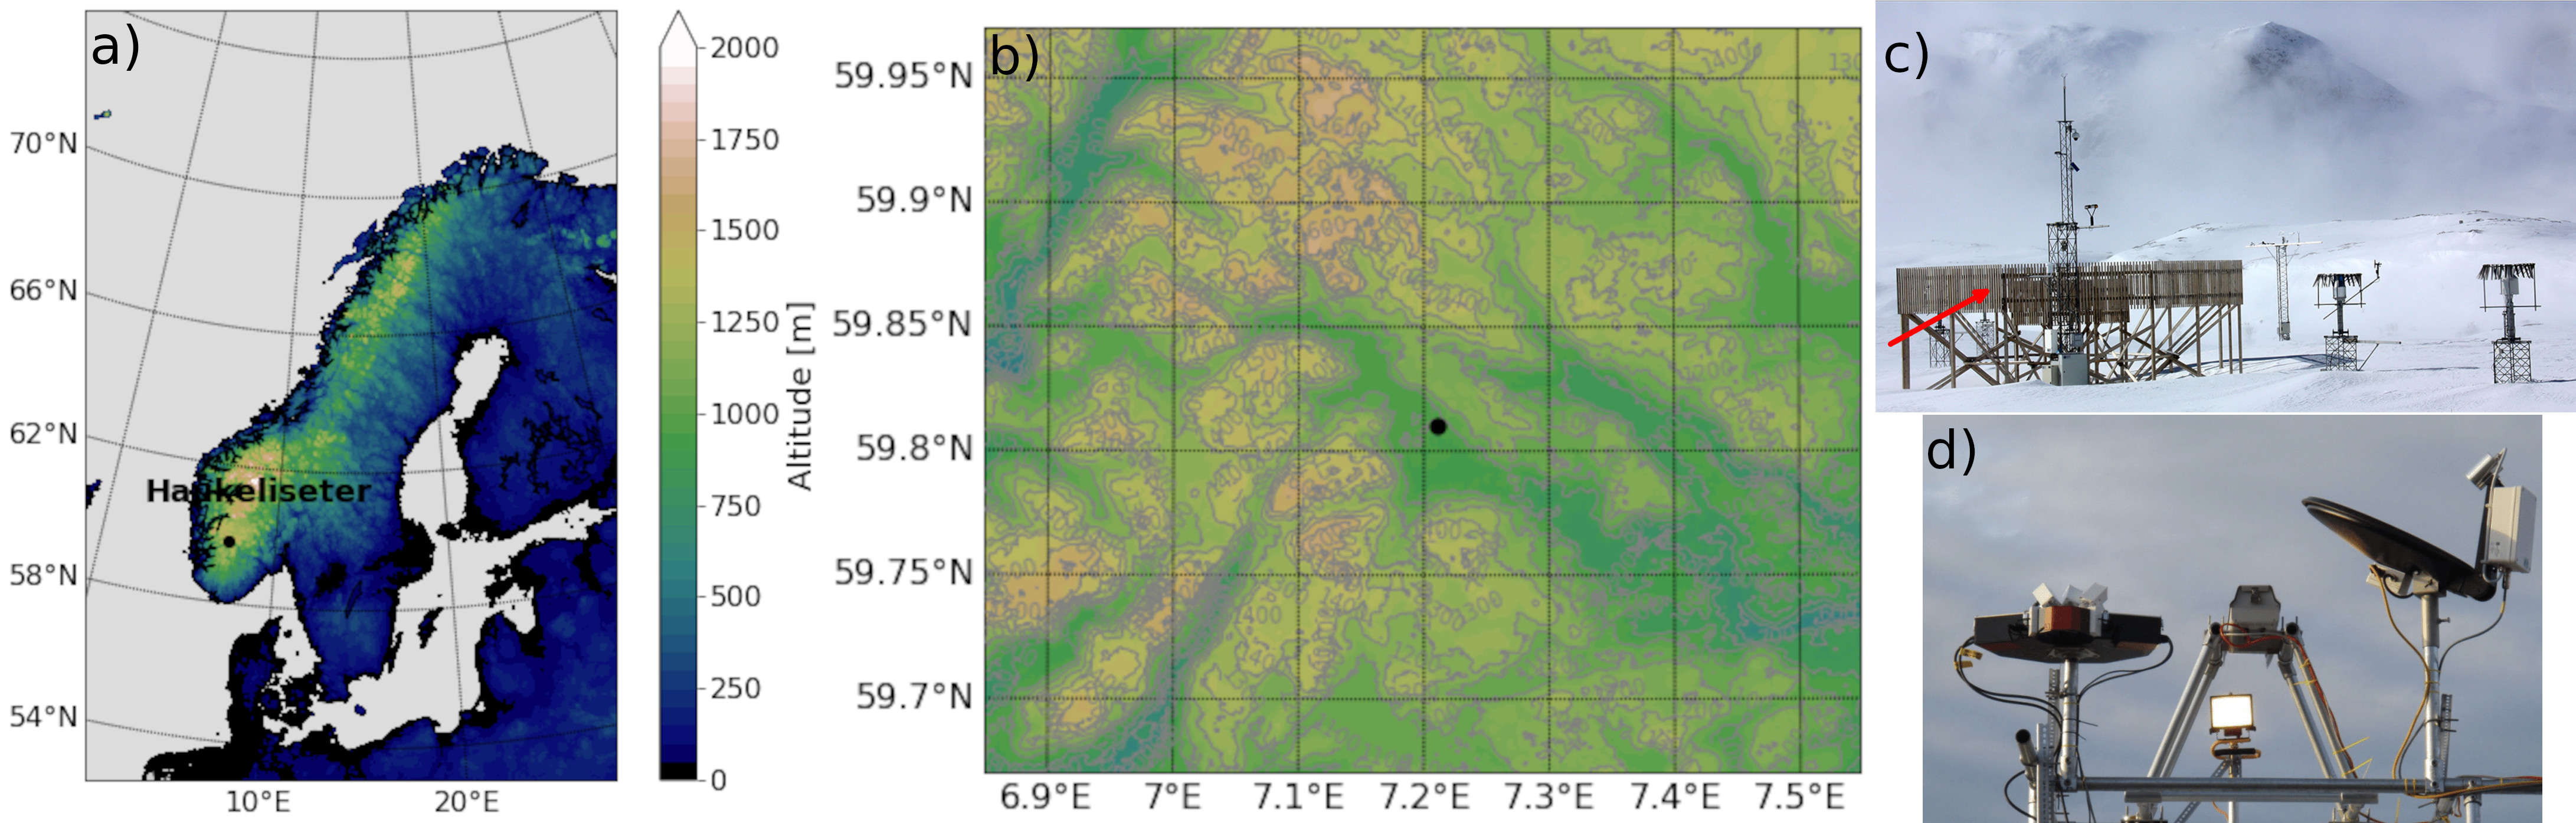
\includegraphics[width=19pc,angle=0]{fig1.jpg}%%%
\DIFdelendFL \DIFaddbeginFL 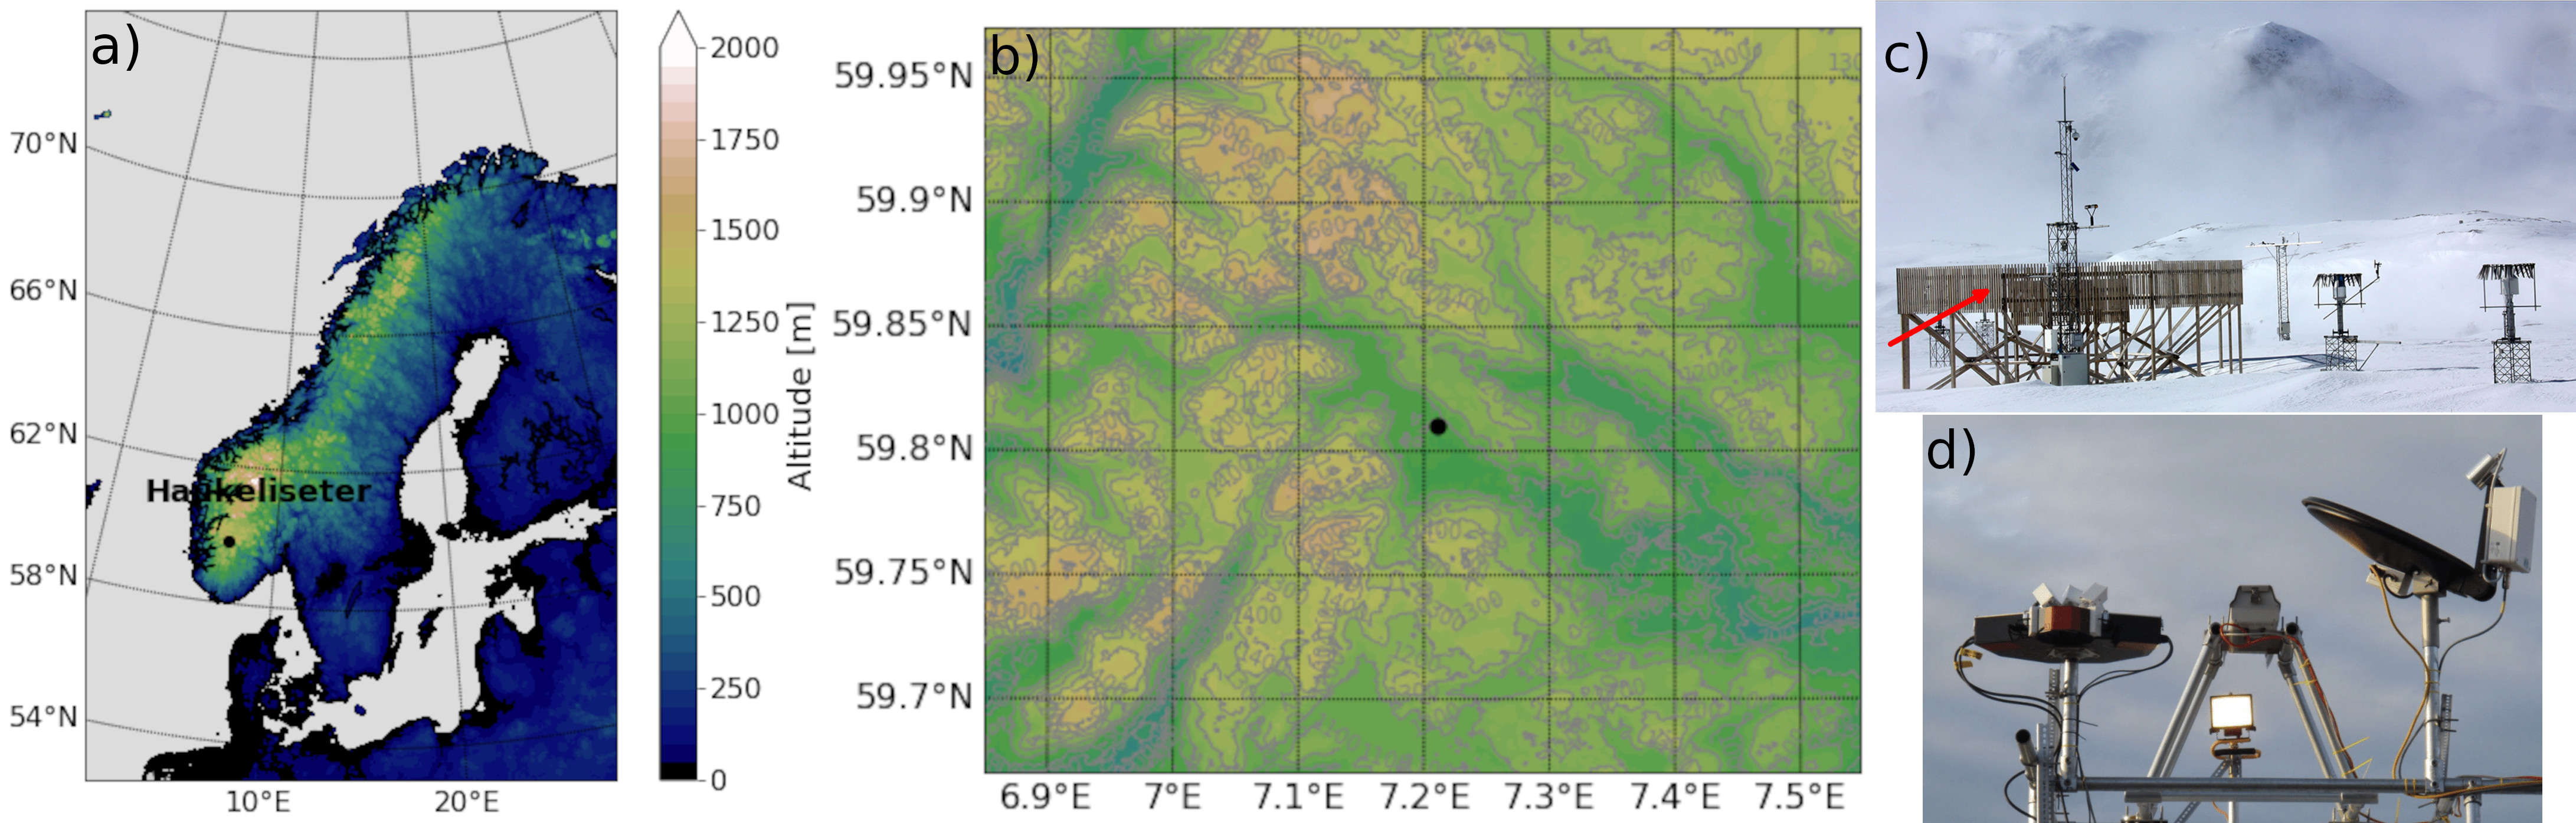
\includegraphics[width=\textwidth,angle=0]{fig1.jpg}\DIFaddendFL \\
	\caption{
		a) Representation of the topography in MEPS and the MEPS model domain. HTS is located in the mountainous region in Southern Norway. The contours and shading present the elevation of the 2.5x2.5\,km grid cells. b) Topographic map around HTS. From the DTM 10 terrain model of \protect\citet{geonorge_dtm_2018}. HTS surrounded by 500\,m higher mountains to the west and more open to the south-east. \DIFaddbeginFL \\ 
		\DIFaddFL{c) DFAR, unprotected precipitation gauges and meteorological mast at HTS. The arrow indicates the westerly wind direction. The figure is adapted from }\protect\DIFaddFL{\mbox{%DIFAUXCMD
\citet{wolff_derivation_2015}}\hspace{0pt}%DIFAUXCMD
. d) Additional instruments installed during HiLaMS during winter 2016-2017: Muli-Angle Snowflake Camera (MASC, left), Precipitation Imaging Package (middle), Micro Rain Radar (MRR, right).
	}\DIFaddendFL }
	\label{fig:norway_map}
\end{figure}


\begin{figure}[t]
	\noindent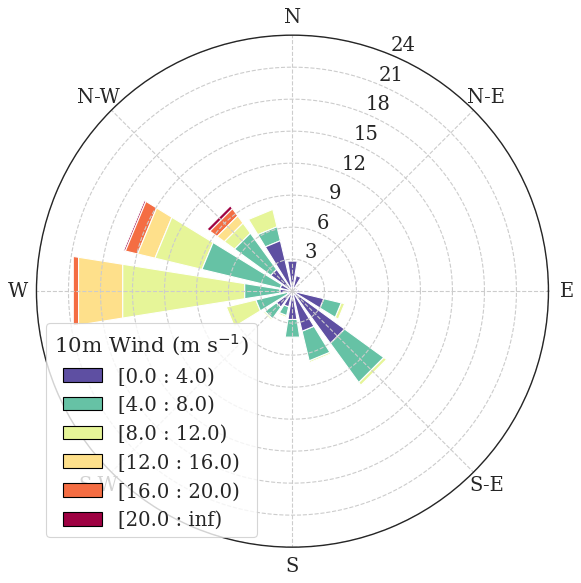
\includegraphics[width=19pc,angle=0]{fig2.png}\\
	\caption{Windrose of the 10-m wind during snowfall events when 24h accumulation $\geq$ 25\,mm\,d$^{-1}$ and 2-m temperature \textless 2\,$^{\circ}$C measured at HTS, during winter 2016-2017. Colors indicate the 10-m wind speed categories used in this study. 
	}
	\label{fig:windrose}
\end{figure}

\begin{figure}[t]
	\noindent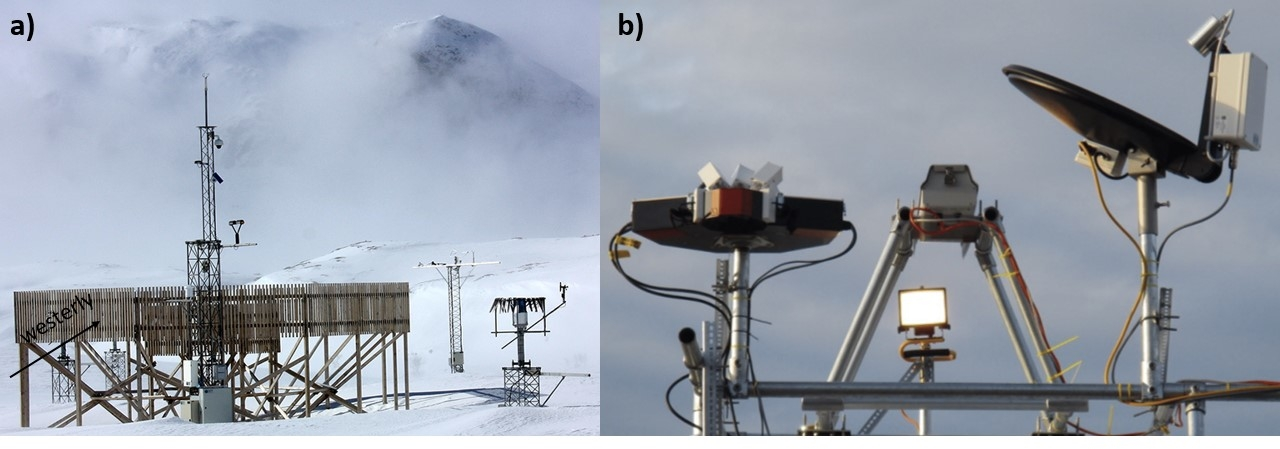
\includegraphics[width=19pc,angle=0]{fig3.jpg}\\
	\caption{
		a) DFAR, unprotected precipitation gauges and meteorological mast at HTS. The arrow indicates the westerly wind direction. The figure is adapted from \protect\citet{wolff_derivation_2015}. b) Additional instruments installed during HiLaMS during winter 2016-2017: \DIFdelbeginFL \DIFdelFL{Muli-Angular }\DIFdelendFL \DIFaddbeginFL \DIFaddFL{Muli-Angle }\DIFaddendFL Snowflake Camera (MASC, left), Precipitation Imaging Package (\DIFdelbeginFL \DIFdelFL{PIP, }\DIFdelendFL middle), Micro Rain Radar (MRR, right).}
	\label{fig:instruments}
\end{figure}

\begin{figure}[t]
	\noindent\DIFdelbeginFL %DIFDELCMD < 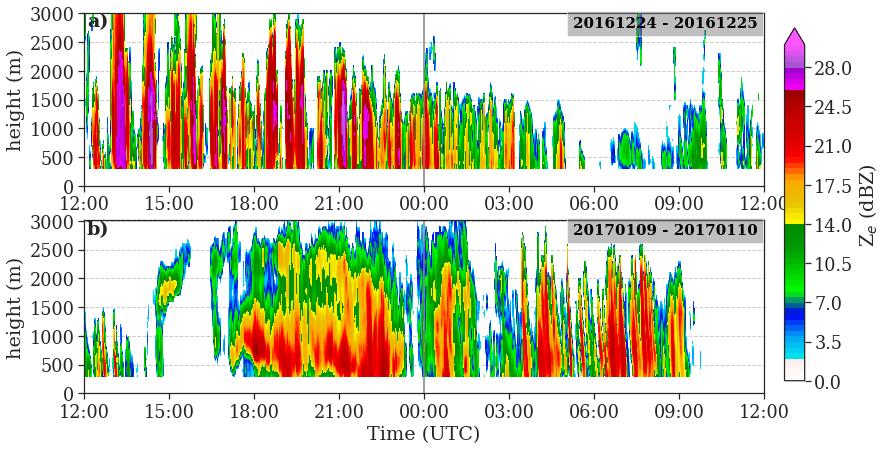
\includegraphics[width=19pc,angle=0]{fig4.png}%%%
\DIFdelendFL \DIFaddbeginFL 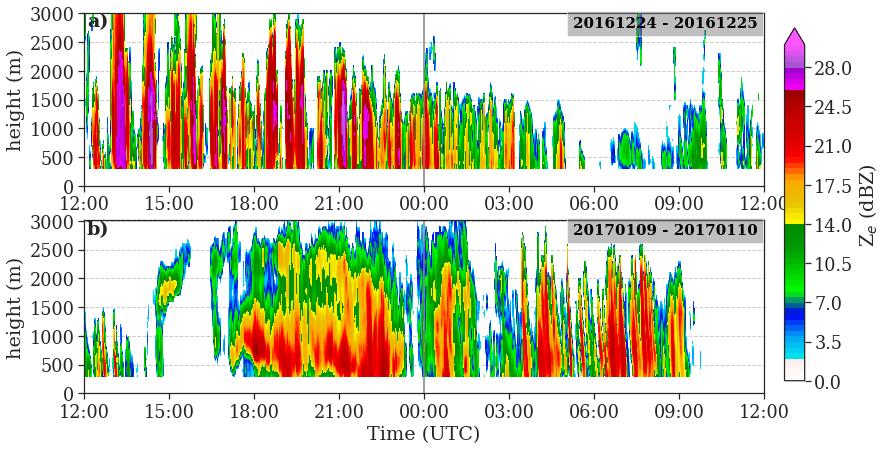
\includegraphics[width=\textwidth,angle=0]{fig4.png}\DIFaddendFL \\
	\caption{Examples of MRR reflectivity during the two typical snowfall regimes. The time series for a westerly snowfall regime case during high wind speed on Dec 24-25 2016 (a). The westerly snowfall regime was associated with interchanging patterns of high and low reflectivities during snowfall. b) example during an easterly snowfall regime with low wind speeds and light precipitation of convective nature, on Jan 09-10 2017.
	}
	\label{fig:MRR_refl}
\end{figure}

\begin{figure}
	\noindent\DIFdelbeginFL %DIFDELCMD < 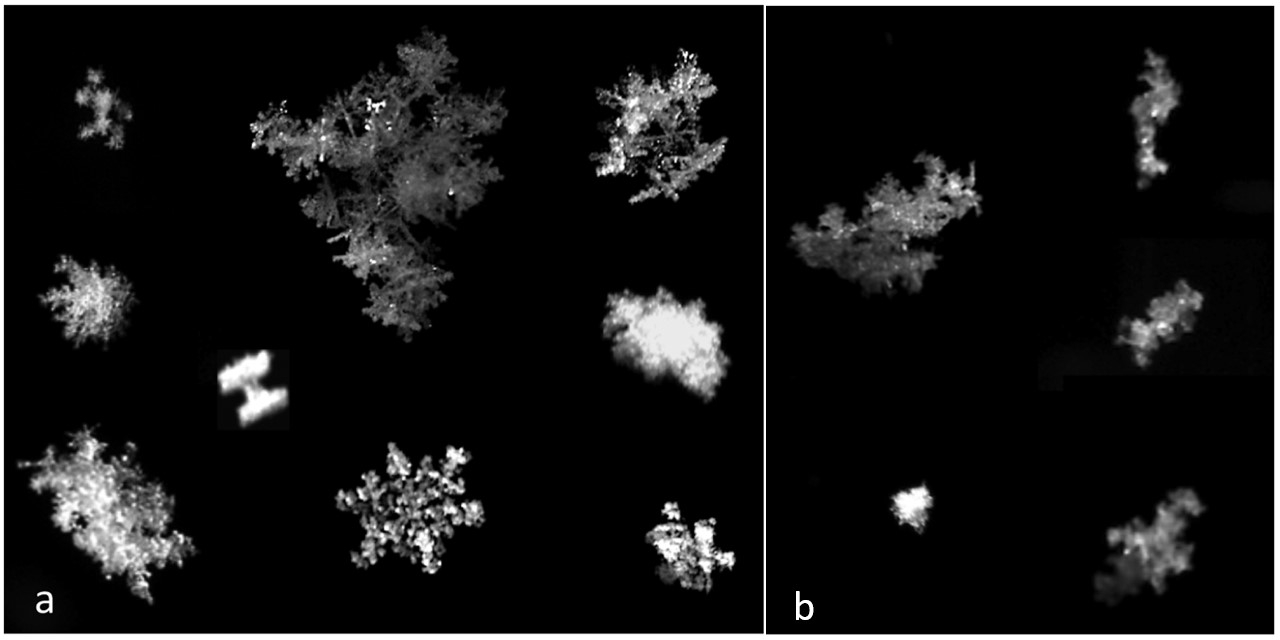
\includegraphics[width=19pc,angle=0]{fig5.jpg}%%%
\DIFdelendFL \DIFaddbeginFL 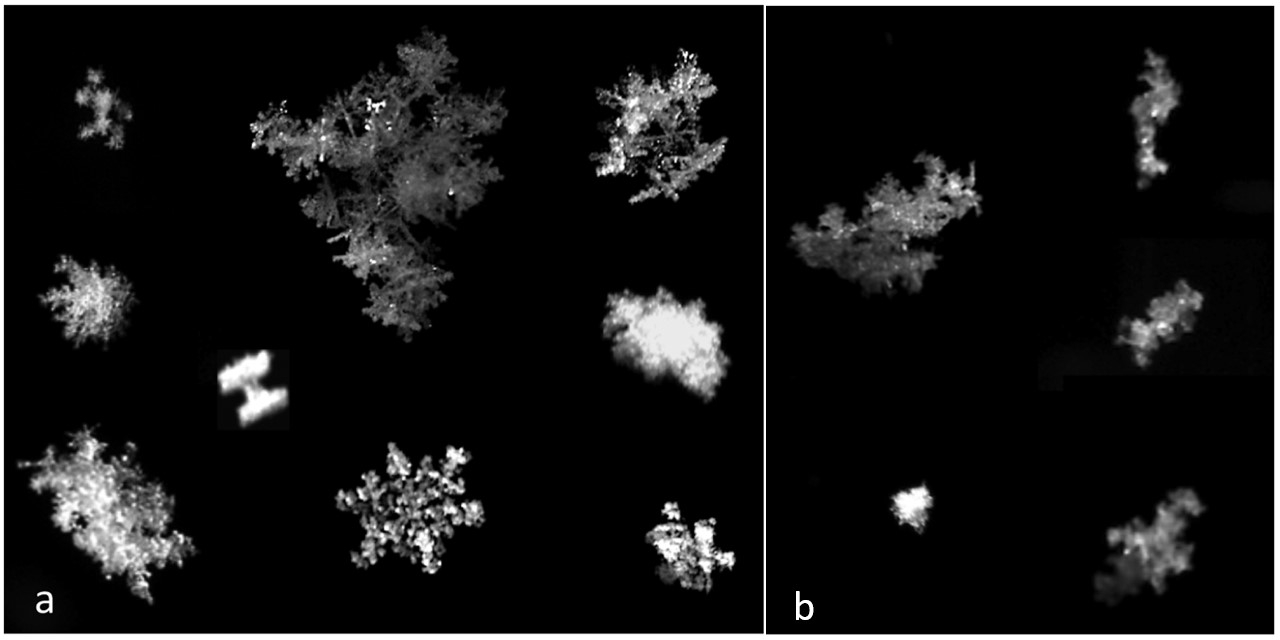
\includegraphics[width=\textwidth,angle=0]{fig5.jpg}\DIFaddendFL \\
	\caption{a) Typical snowflake habits observed during events classified in the easterly snowfall regime. b) Examples of large precipitating crystals observed during the westerly snowfall regime. This figure is adapted from \protect\citet{schirle_estimation_2019}.
	}
	\label{fig:snowflakes}
\end{figure}

\begin{figure}
	\noindent\DIFdelbeginFL %DIFDELCMD < 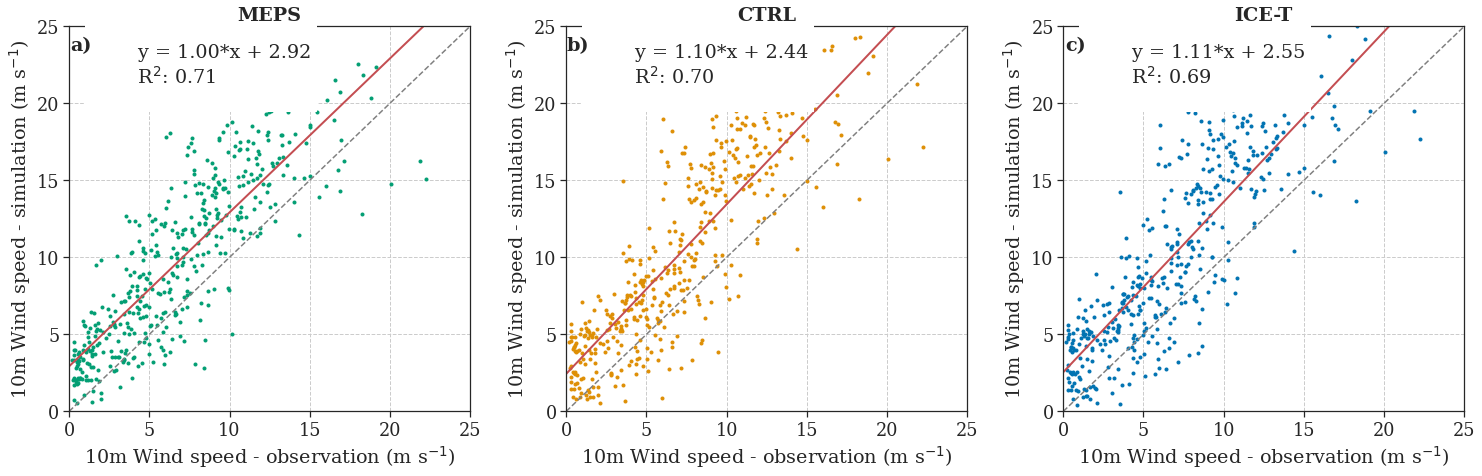
\includegraphics[width=19pc,angle=0]{fig6.png}%%%
\DIFdelendFL \DIFaddbeginFL 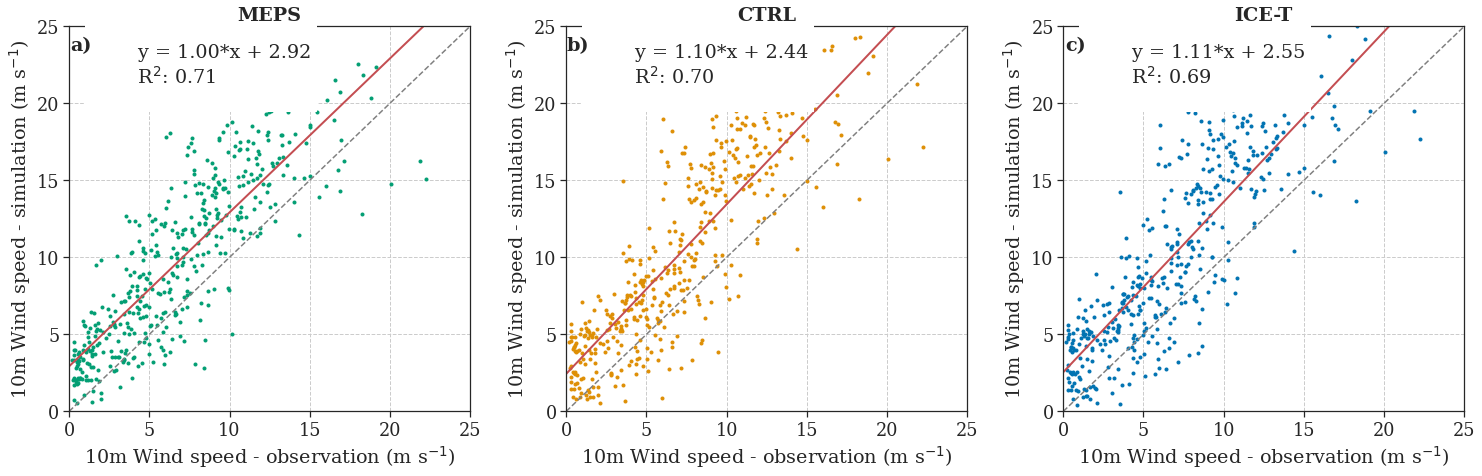
\includegraphics[width=\textwidth,angle=0]{fig6.png}\DIFaddendFL \\
	\caption{Known 10-m wind bias \citep{frogner_convection-permitting_2019} was reduced according to the correlation equation between 10-m wind speeds observed at the DFAR and MEPS, CTRL, and ICE-T in a, b, and c, respectively. The red line indicates the linear correlation between DFAR and OESR. \DIFaddbeginFL \DIFaddFL{The grey dashed lines represent the line of equality where model simulations are equal to observations. 
	}\DIFaddendFL }
	\label{fig:WS_correlation}
\end{figure}

\begin{figure}
	\noindent\DIFdelbeginFL %DIFDELCMD < 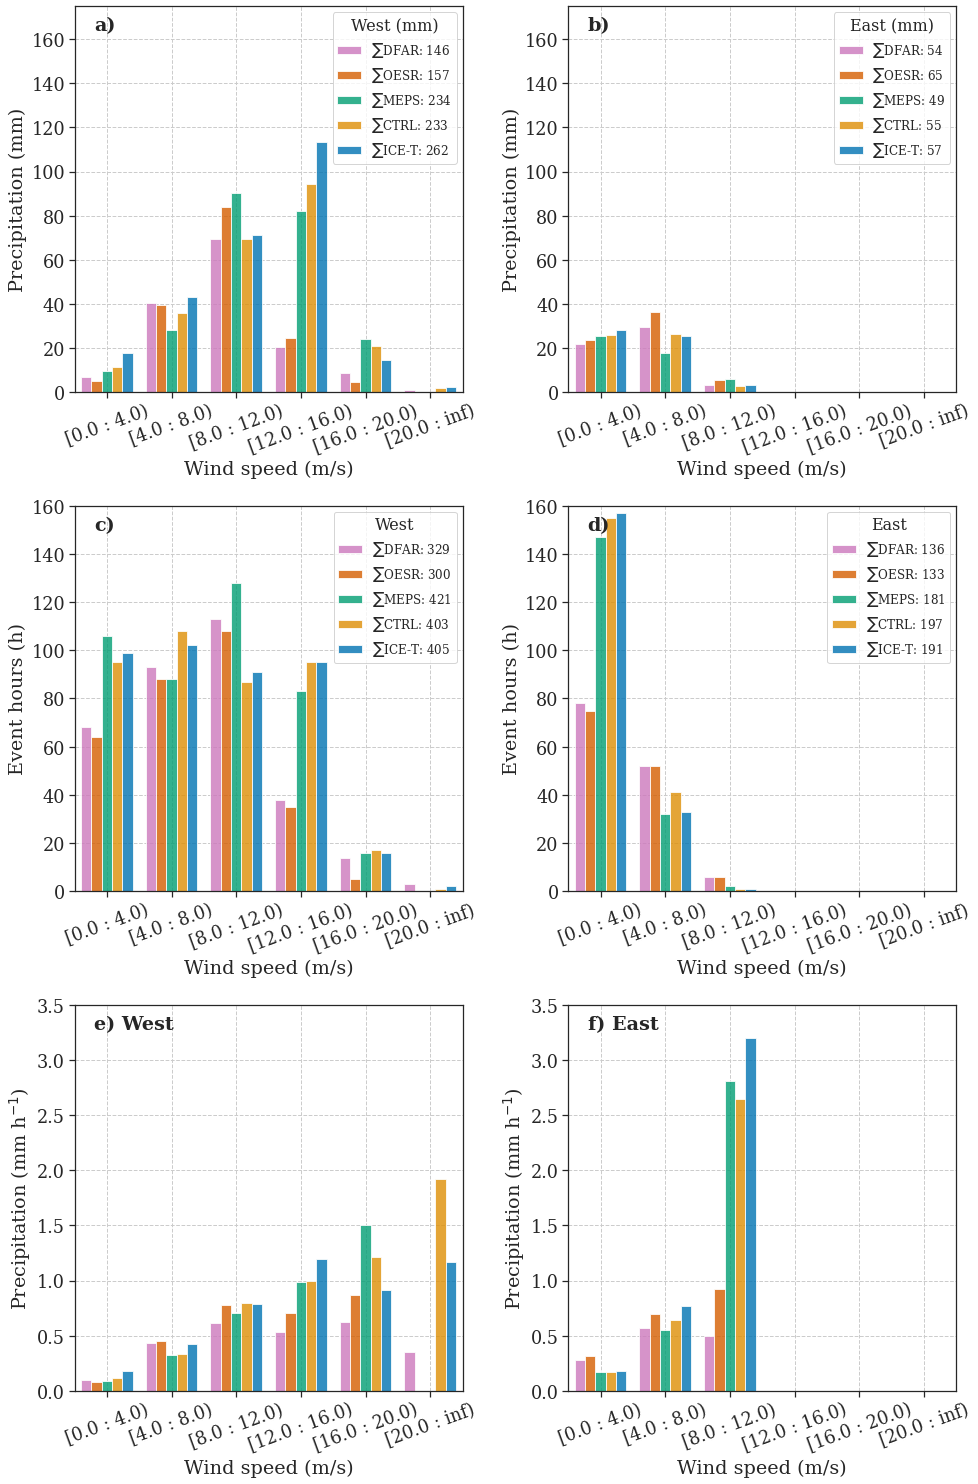
\includegraphics[width=19pc,angle=0]{fig7.png}%%%
\DIFdelendFL \DIFaddbeginFL 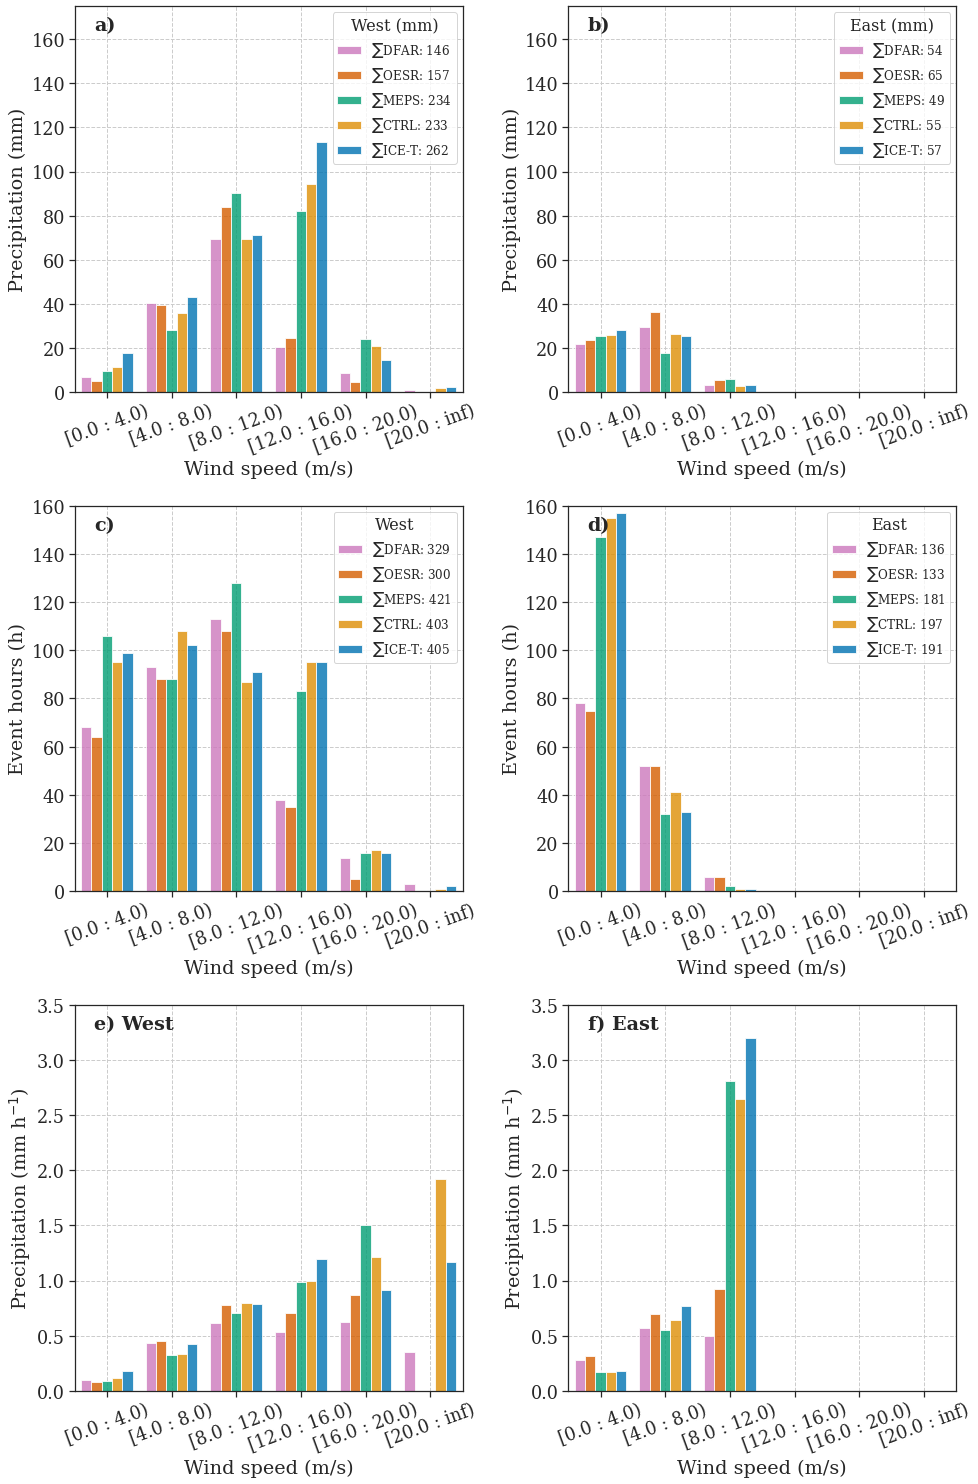
\includegraphics[width=0.65\textwidth,angle=0]{fig7.png}\DIFaddendFL \\
	\caption{Surface snowfall accumulation for DFAR observations, OESR, MEPS, CTRL, and ICE-T separated into westerly (a) and easterly (b) snowfall regimes for 27 precipitation days during winter 2016-2017. The sum \DIFaddbeginFL \DIFaddFL{($\sum$) over the 27 days }\DIFaddendFL of total precipitation accumulation in each snowfall regime is presented in the figure \DIFdelbeginFL \DIFdelFL{label }\DIFdelendFL \DIFaddbeginFL \DIFaddFL{legend }\DIFaddendFL in a\DIFaddbeginFL \DIFaddFL{) }\DIFaddendFL and b\DIFaddbeginFL \DIFaddFL{)}\DIFaddendFL . The separation into wind speed regimes is done for the corrected simulated wind according to the correlation equation in Fig. \ref{fig:WS_correlation} for MEPS, CTRL, and ICE-T. c\DIFaddbeginFL \DIFaddFL{) }\DIFaddendFL and d\DIFaddbeginFL \DIFaddFL{) }\DIFaddendFL show the event hours observed at the DFAR and OESR as well as the simulated precipitation hours in the NWPs. The total sum \DIFaddbeginFL \DIFaddFL{($\sum$) }\DIFaddendFL of the precipitation hours is presented in the figure label for the 27 precipitation days. Further, the snowfall accumulation is divided by the event hours in e) and f) for westerly and easterly, respectively.
	}
	\label{fig:sfc_WS_WD}
\end{figure}

\begin{figure}
	\noindent\DIFdelbeginFL %DIFDELCMD < 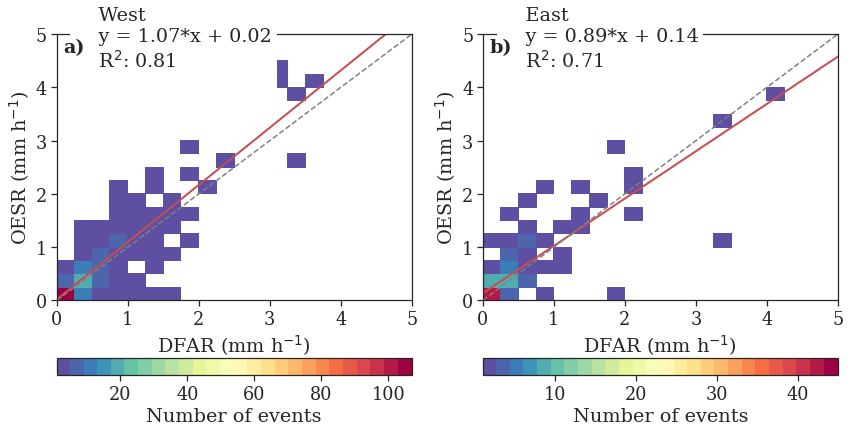
\includegraphics[width=19pc,angle=0]{fig8.png}%%%
\DIFdelendFL \DIFaddbeginFL 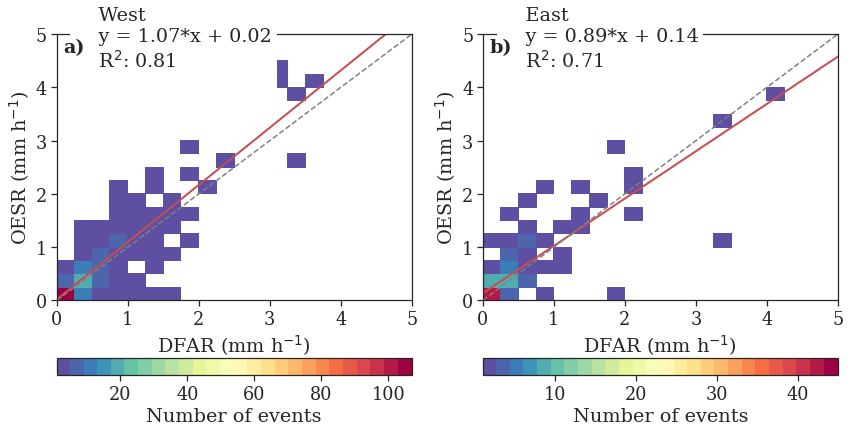
\includegraphics[width=\textwidth,angle=0]{fig8.png}\DIFaddendFL \\
	\caption{Surface snowfall validation of OESR of the hourly snowfall accumulation, with DFAR observations on the x-axis and OESR estimates on the y-axis. The hourly accumulated snowfall amount is separated into westerly snowfall regime in a, and easterly snowfall regime in b. The red line indicates the linear correlation between the DFAR and the OESR surface snowfall accumulation. During westerly snowfall 121 events were counted at the 0.1\,mm\,h$^{-1}$ bin, while during easterly only 45 events were counted at the 0.1\,mm\,h$^{-1}$ bin. \DIFaddbeginFL \DIFaddFL{The grey dashed lines represent the line of equality where OESR are equal to observations.
	}\DIFaddendFL }
	\label{fig:sfc_oesr}
\end{figure}


\begin{figure}
	\noindent\DIFdelbeginFL %DIFDELCMD < 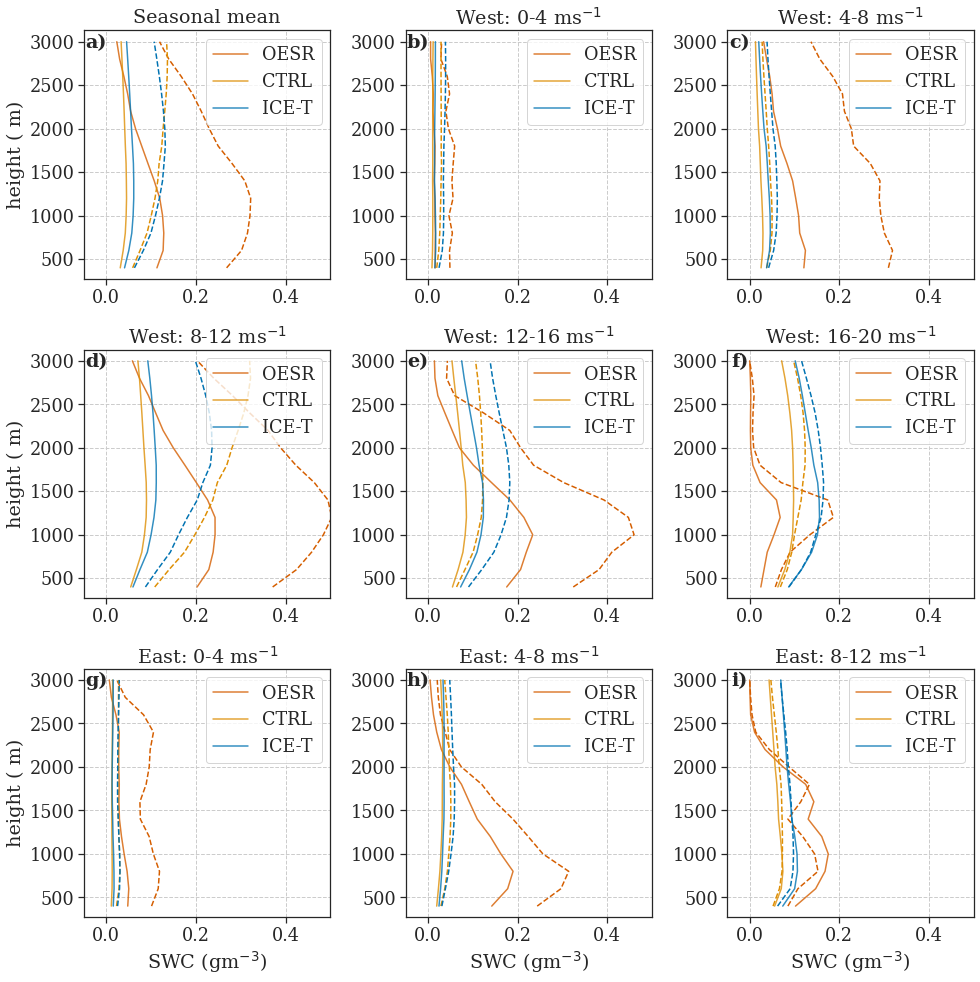
\includegraphics[width=19pc,angle=0]{fig9.png}%%%
\DIFdelendFL \DIFaddbeginFL 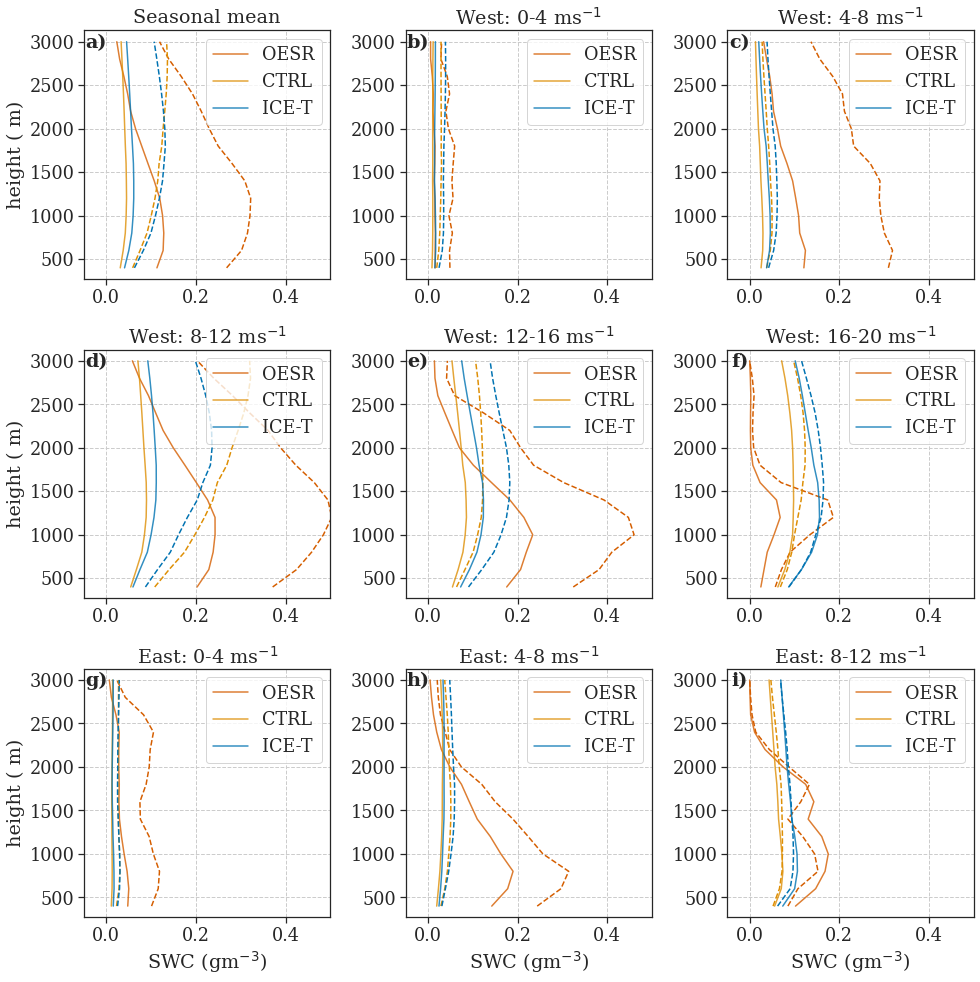
\includegraphics[width=\textwidth,angle=0]{fig9.png}\DIFaddendFL \\
	\caption{Mean (solid) and standard deviation (dashed) of instantaneous SWC separated into west (a-f), east (g-i) snowfall regimes for days fulfilling the analysis requirements during winter 2016-2017. The SWC is sorted into snowfall regimes with the adjusted wind speed correction from the correlation equation in Fig. \ref{fig:WS_correlation}b and c for CTRL and ICE-T, respectively.
	}
	\label{fig:vert_swc}
\end{figure}


\begin{figure}
	\noindent\DIFdelbeginFL %DIFDELCMD < 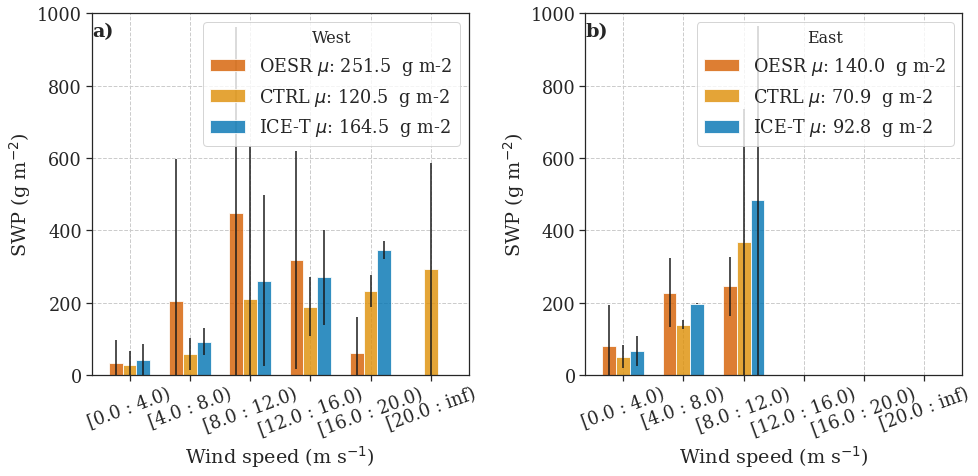
\includegraphics[width=19pc,angle=0]{fig10.png}%%%
\DIFdelendFL \DIFaddbeginFL 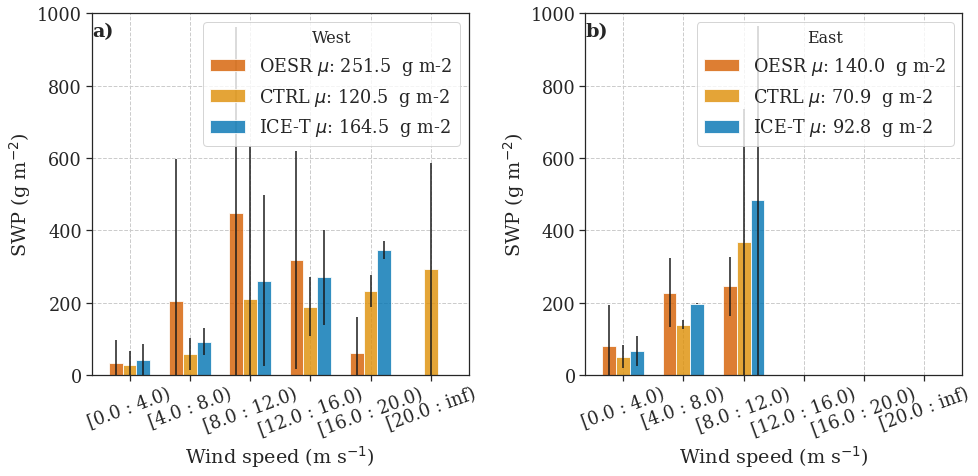
\includegraphics[width=\textwidth,angle=0]{fig10.png}\DIFaddendFL \\
	\caption{Seasonal mean of instantaneous SWP for OESR, CTRL, and ICE-T forecasts separated into westerly and easterly snowfall regimes in a and b, respectively for 27 precipitation days during winter 2016-2017. The separation into wind speed is done with the corrected wind speed bias from Fig. \ref{fig:WS_correlation}b and c for CTRL and ICE-T, respectively. The black line indicates the standard deviation ($\pm \sigma$) in each snowfall wind regime. The mean and standard deviation in each wind speed bin is calculated individually hence the result is dependent on the event hours. The figure labels show the total mean of SWP for over all wind \DIFdelbeginFL \DIFdelFL{speed }\DIFdelendFL \DIFaddbeginFL \DIFaddFL{speeds }\DIFaddendFL and all precipitation event hours. 
	%DIF < mean SWP per hour
}
	\label{fig:swp_WS_WD}
\end{figure}
%DIF < 
 \DIFaddbegin 


 \DIFaddend\end{document}